\documentclass[10pt,a4paper%,twoside,openright,titlepage,fleqn,%
% headinclude,footinclude,BCOR5mm,%
% numbers=noenddot,cleardoublepage=empty,%
tablecaptionabove]{article}

\usepackage{geometry}
\geometry{left=2.5cm,right=2.5cm,top=2.5cm,bottom=2.5cm}
\usepackage{subfigure}
\usepackage{amsmath,amssymb,amsthm}

%% -----------------设置数学公式字体-------------------------
%% Font style 1
%% \newcommand\ibinom[2]{\genfrac\lbrace\rbrace{0pt}{}{#1}{#2}}
%% \usepackage{bm}

%% Font style 2
%% \newcommand\ibinom[2]{\genfrac\lbrace\rbrace{0pt}{}{#1}{#2}} 
%% \usepackage[boldsans]{ccfonts} 
%% \usepackage{bm} 

%% Font style 3
\newcommand\ibinom[2]{\genfrac\lbrace\rbrace{0pt}{}{#1}{#2}}
\usepackage[euler-digits]{eulervm}
\usepackage{bm}

%% Font style 4
%% \usepackage{fourier}
%% \newcommand\ibinom[2]{\genfrac\lbrace\rbrace{0pt}{}{#1}{#2}}
%% \usepackage{bm}

%% Font style 5
%% \newcommand\ibinom[2]{\genfrac\lbrace\rbrace{0pt}{}{#1}{#2}}
%% \usepackage{mathptmx}
%% \usepackage{bm} 


%% %% Font style 6
%% \newcommand\ibinom[2]{\genfrac\lbrace\rbrace{0pt}{}{#1}{#2}}
%% \usepackage{txfonts}
%% \usepackage{bm}
%% -----------------------------------------------------------
%% \usepackage[T1]{fontenc} % Needed for Type1 Concrete
%% %% \usepackage{concrete} % Loads Concrete + Euler VM
%% %% \usepackage{pxfonts} % Or palatino or mathpazo
%% \usepackage{eulervm} %
%% %% \usepackage{kerkis} % Kerkis roman and sans
%% %% \usepackage{kmath} % Kerkis math
%% \usepackage{fourier}
\usepackage{pgf}
\usepackage{tikz}
\usetikzlibrary{calc}
\usetikzlibrary{arrows,snakes,backgrounds,shapes}
\usetikzlibrary{matrix,fit,positioning,decorations.pathmorphing}
\usepackage{CJK} 
\usepackage{amsmath,amssymb,amsfonts}
\usepackage{mathdots}
\usepackage{subfigure}
\usepackage{caption}
\usepackage{verbatim,color,xcolor}
\usepackage{graphicx}
\usepackage{manfnt}
\usepackage{fancybox}
\usepackage{textcomp}
\usepackage{multirow,multicol}
\usepackage{parcolumns}
\usepackage{framed}
\usepackage{threeparttable}
\usepackage{extarrows}
\usepackage{listings}
\lstset{
  keywordstyle=\color{blue!70},
  frame=lines,
  basicstyle=\ttfamily\small,
  commentstyle=\small\color{red},
  rulesepcolor=\color{red!20!green!20!blue!20},
  tabsize=4,
  numbersep=5pt,
  backgroundcolor=\color[rgb]{0.95,1.0,1.0},
  showspaces=false,
  showtabs=false,
  extendedchars=false,
  escapeinside=``
}
%% \usepackage[utf8]{inputenc}
%% \usepackage[upright]{fourier}   %

%%%% \renewcommand *****
\renewcommand{\lstlistingname}{}
\newcommand{\tf}{\ttfamily}
\newcommand{\ttt}{\texttt}
\newcommand{\blue}{\textcolor{blue}}
\newcommand{\red}{\textcolor{red}}
\newcommand{\purple}{\textcolor{purple}}
\newcommand{\ft}{\frametitle}
\newcommand{\bs}{\boldsymbol}
\newcommand{\disp}{\displaystyle}
\newcommand{\ds}{\displaystyle}
\newcommand{\vd}{\vdots}
\newcommand{\cd}{\cdots}
\newcommand{\dd}{\ddots}
\newcommand{\id}{\iddots}
\newcommand{\XX}{\mathbf{X}}
\newcommand{\PP}{\mathbf{P}}
\newcommand{\QQ}{\mathbf{Q}}
\newcommand{\xx}{\mathbf{x}}
\newcommand{\yy}{\mathbf{y}}
\newcommand{\bb}{\mathbf{b}}
\newcommand{\aaa}{\mathbf{a}}
\newcommand{\A}{\mathbf{A}}
\newcommand{\B}{\mathbf{B}}
\newcommand{\C}{\mathbf{C}}
\newcommand{\D}{\mathbf{D}}
\newcommand{\E}{\mathbf{E}}
\newcommand{\U}{\mathbf{U}}
\newcommand{\X}{\mathbf{X}}
\newcommand{\Y}{\mathbf{Y}}
\newcommand{\Z}{\mathbf{Z}}
\newcommand{\T}{\mathbf{T}}
\newcommand{\zero}{\mathbf{0}}
\newcommand{\II}{\mathbf{I}}
\newcommand{\ii}{\mathbf{i}}
\newcommand{\jj}{\mathbf{j}}
\newcommand{\kk}{\mathbf{k}}
\newcommand{\uu}{\mathbf{u}}
\newcommand{\vv}{\mathbf{v}}
\newcommand{\ee}{\mathbf{e}}
\newcommand{\Lambdabd}{\mathbf{\Lambda}}
\newcommand{\alphabd}{\boldsymbol{\alpha}}
\newcommand{\betabd}{\boldsymbol{\beta}}
\newcommand{\gammabd}{\boldsymbol{\gamma}}
\newcommand{\xibd}{\boldsymbol{\xi}}
\newcommand{\epsilonbd}{\boldsymbol{\epsilon}}
\newcommand{\etabd}{\boldsymbol{\eta}}
\newcommand{\rr}{\mathrm{r}}
\newcommand{\RR}{\mathrm{R}}
\newcommand{\RRR}{\mathbb{R}}
\newcommand{\CCC}{\mathbb{C}}


\begin{document}

\begin{CJK}{UTF8}{gkai}
  \pagenumbering{roman}
  \pagestyle{plain}
  \pagenumbering{arabic}
  
  \renewcommand{\proofname}{\textbf{证明}}
  \renewcommand{\figurename}{\textbf{图}}

  \renewcommand{\proofname}{\textbf{证明}}
\newtheorem{li}{例}
\newtheorem{lianxi}{练习}
\newtheorem{jielun}{结论}
\newtheorem{dingli}{定理}
\newtheorem{mingti}{{命题}} 
\newtheorem{yinli}{{引理}} 
\newtheorem{tuilun}{{推论}}
\newtheorem{dingyi}{{定义}} 
\newtheorem{example}{{例}}
\newtheorem*{li*}{{例}}
\newtheorem*{jie}{{解}}
\newtheorem*{zhengming}{{证明}}
\newtheorem{zhu}{{注}}
\newtheorem*{zhu*}{{注}}
\newtheorem{xingzhi}{{性质}}
\newtheorem{wenti}{{问题}}
\newtheorem{rem}{{Remark}}
\newtheorem{lem}{{Lemma}}


  \title{第3讲、向量组}
  % \author{张晓平}
  % \date{}           % Activate to display a given date or no date
  \maketitle

  %%%%%
\section{$n$维向量及其线性相关性}

考察三元齐次线性方程组
\begin{equation}\label{ls}
  \left\{
  \begin{array}{l}
    a_{11}x_1+a_{12}x_2+a_{13}x_3=0,\\[0.1in]
    a_{21}x_1+a_{22}x_2+a_{23}x_3=0,\\[0.1in]
    a_{31}x_1+a_{32}x_2+a_{33}x_3=0
  \end{array}
  \right.
\end{equation}
我们用向量工具给出其几何解释。
记
$$
\ii = \left(
\begin{array}{ccc}
  1&
  0&
  0
\end{array}
\right), ~~
\jj = \left(
\begin{array}{ccc}
  0&
  1&
  0
\end{array}
\right), ~~
\kk = \left(
\begin{array}{ccc}
  0&
  0&
  1
\end{array}
\right),
$$
则
$$
\alphabd_i = \left(
\begin{array}{ccc}
  a_{i1}&
  a_{i2}&
  a_{i3}
\end{array}
\right) = a_{i1} \ii + a_{i2} \jj + a_{i3} \kk, \quad i=1,2,3,
$$
且
$$
\xx = \left(
\begin{array}{ccc}
  x_1&
  x_2&
  x_3
\end{array}
\right) = x_1\ii + x_2\jj + x_3\kk
$$


\begin{dingyi}[向量的内积]
  两个向量$\uu=(u_1,u_2,u_3), ~~\vv=(v_1,v_2,v_3)$的内积定义为
  $$
  (\uu,\vv)=u_1v_1+u_2v_2+u_3v_3.
  $$
\end{dingyi}

\begin{dingyi}[向量的垂直]
  两个向量$\uu=(u_1,u_2,u_3), ~~\vv=(v_1,v_2,v_3)$垂直的充分必要条件是
  $$
  (\uu,\vv)=0.
  $$
\end{dingyi}


由以上方程组可看出,解向量$\xx$与$\alphabd_1,\alphabd_2,\alphabd_3$都垂直。 故
\begin{itemize}
\item[(1)] 若$\alphabd_1,\alphabd_2,\alphabd_3$不共面,只有零向量与三者都垂直,即线性方程组(\ref{ls})只有零解;
\item[(2)] 若$\alphabd_1,\alphabd_2,\alphabd_3$共面但不共线,则与该平面垂直的向量都是线性方程组(\ref{ls})的解,
  故(\ref{ls})有无穷多个彼此平行的解向量;
\item[(3)] 若$\alphabd_1,\alphabd_2,\alphabd_3$共线,则过原点且与该直线垂直的平面上的全体向量都是(\ref{ls})的解向量,
  此时任一解向量均可表示为
  $$
  \xx = k_1 \xx^{(1)} + k_2 \xx^{(2)},
  $$
  其中$\xx^{(1)}, \xx^{(2)}$为(\ref{ls})的某两个不共线的非零解向量,$k_1,k_2$为任意常数。
\end{itemize}


\begin{dingyi}[$n$维向量]
  数域$F$上的$n$个数$a_1,a_2,\cd,a_n$构成的有序数组称为数域$F$上的一个$n$维向量,记为
  \begin{equation}\label{vec}
    \alphabd = (a_1, a_2, \cd, a_n)
  \end{equation}
  其中$a_i$称为$\alphabd$的第$i$个分量。
\end{dingyi}


\begin{itemize}
\item 形如(\ref{vec})的向量称为\red{行向量};
\item 形如
  $$
  \alphabd = (a_1, a_2, \cd, a_n)^T = \left(
  \begin{array}{c}
    a_1\\
    a_2\\
    \vd\\
    a_n
  \end{array}
  \right)
  $$
  的向量称为\red{列向量}。
\end{itemize}


数域$F$上全体$n$维向量组成的集合,记作$F^n$。 设$\alphabd\in F^n$,则
\begin{itemize}
\item 当$F$取为$\mathbb R$时,$\alphabd$为实向量;
\item 当$F$取为$\mathbb C$时,$\alphabd$为复向量。
\end{itemize}






\begin{dingyi}{向量运算}
  设$\alphabd=(a_1,a_2,\cd,a_n),~~\betabd=(b_1,b_2,\cd,b_n)\in F^n$,$k\in F$,定义
  \begin{enumerate}
  \item[(i)]
    $\alphabd=\betabd$当且仅当$a_i=b_i(i=1,2,\cd,n)$;
  \item[(ii)] 向量加法
    $$
    \alphabd+\betabd=(a_1+b_1,a_2+b_2,\cd,a_n+b_n)
    $$
  \item[(iii)] 向量数乘
    $$
    k\alphabd=(ka_1,ka_2,\cd,ka_n)
    $$
  \end{enumerate}
\end{dingyi}


\begin{itemize}
\item 在$(iii)$中取$k=-1$,得
  $$
  (-1)\alphabd = (-a_1,-a_2,\cd,-a_n)
  $$
  右端的向量称为$\alphabd$的负向量,记为$-\alphabd$. 
\item 向量的减法定义为
  $$
  \betabd-\alphabd = \betabd + (-\alphabd)
  $$
\end{itemize}

\begin{dingyi}[向量的8条运算规则]
  设$\alphabd,\betabd,\gammabd\in F^n, 1,k,l\in F$,则
  \begin{itemize}
  \item[(1)] $\alphabd+\betabd=\betabd+\alphabd$
  \item[(2)] $(\alphabd+\betabd)+\gammabd=\alphabd+(\betabd+\gammabd)$
  \item[(3)] 对任一向量$\alphabd$,有$\alphabd+\zero=\alphabd$
  \item[(4)] 对任一向量$\alphabd$,存在负向量$-\alphabd$,使得$\alphabd+(-\alphabd)=\zero$
  \item[(5)] $1\alphabd=\alphabd$
  \item[(6)] $k(l\alphabd)=(kl)\alphabd$
  \item[(7)] $k(\alphabd+\betabd)=k\alphabd+k\betabd$
  \item[(8)] $(k+l)\alphabd=k\alphabd+l\alphabd$
  \end{itemize}
\end{dingyi}

\begin{dingyi}[向量空间]
  数域$F$上的$n$维向量,在其中定义了上述加法与数乘运算,就称之为$F$上的$n$维向量空间,仍记为$F^n$。
  当$F=\mathbb R$时,叫做$n$维实向量空间,记作$\mathbb R^n$。
\end{dingyi}

\begin{dingyi}[线性表示]
  设$\alphabd_i\in F^n, k_i \in F (i=1,2,\cd,m)$,则向量
  $$
  \sum_{i=1}^m k_i\alphabd_i = k_1\alphabd_1 + k_2\alphabd_2+\cd + k_m\alphabd_m
  $$
  称为向量组$\alphabd_1,\alphabd_2,\cd,\alphabd_m$在数域$F$上的一个\red{线性组合}。  如果记
  $$\betabd=\sum_{i=1}^m k_i\alphabd_i,$$
  则称$\betabd$可由$\alphabd_1,\alphabd_2,\cd,\alphabd_m$\red{线性表示}(或\red{线性表出})。
\end{dingyi}


设有线性方程组$\A\xx=\bb$,其中$\A$为$m\times n$矩阵。记
$$\A=(\alphabd_1,\alphabd_2,\cd,\alphabd_n),$$
即
$$
(\alphabd_1,\alphabd_2,\cd,\alphabd_n) \left(
\begin{array}{c}
  x_1\\
  x_2\\
  \vd\\
  x_n
\end{array}
\right)=\bb
$$
于是线性方程组可等价的表述为
$$
x_1\alphabd_1+x_2\alphabd_2+\cd+x_n\alphabd_n=\bb
$$
\begin{zhu*}
  向量$\bb$可由$\alphabd_1,\alphabd_2,\cd,\alphabd_n$线性表示,等价于方程组
  $$
  x_1\alphabd_1+x_2\alphabd_2+\cd+x_n\alphabd_n=\bb
  $$
  有解。
\end{zhu*}

\begin{dingyi}[线性相关与线性无关]
  若对$m$个向量$\alphabd_1,\alphabd_2,\cd,\alphabd_m\in F^n$,有$m$个不全为零的数$k_1,k_2,\cd,k_m\in F$,使
  \begin{equation}\label{def1}
    k_1\alphabd_1 + k_2\alphabd_2+\cd + k_m\alphabd_m = \zero        
  \end{equation}
  成立,则称\red{$\alphabd_1,\alphabd_2,\cd,\alphabd_m$线性相关};
  否则,称\red{$\alphabd_1,\alphabd_2,\cd,\alphabd_m$线性无关}。
\end{dingyi}


\begin{zhu*}
  向量组$\alphabd_1,\alphabd_2,\cd,\alphabd_m$线性无关,指的是
  \begin{itemize}
  \item 没有不全为零的数$k_1,k_2,\cd,k_m$使(\ref{def1})成立 
  \item 只有当$k_1,k_2,\cd,k_m$全为零时,才使(\ref{def1})成立 
  \item 若(\ref{def1})成立,则$k_1,k_2,\cd,k_m$必须全为零
  \end{itemize}
\end{zhu*}



\begin{dingli}
  以下两组等价关系成立:
  \begin{itemize}
  \item  向量组$\alphabd_1,\alphabd_2,\cd,\alphabd_m$线性相关,等价于齐次方程组
    $$
    x_1\alphabd_1+x_2\alphabd_2+\cd+x_m\alphabd_m=\zero
    $$
    有非零解。
  \item  向量组$\alphabd_1,\alphabd_2,\cd,\alphabd_m$线性无关,等价于齐次方程组
    $$
    x_1\alphabd_1+x_2\alphabd_2+\cd+x_m\alphabd_m=\zero
    $$
    只有零解。
  \end{itemize}

\end{dingli}

对于只含有一个向量$\alphabd$的向量组,若存在不为零的数$k$使得
$$
k \alphabd = \zero,
$$
则
$$
\Rightarrow \alphabd = \frac1k \zero = \zero
$$  
若$\alphabd\ne \zero$,要使
$$
k \alphabd = \zero,
$$
必须$k=0$.

\begin{itemize}
\item 当$\alphabd=\zero$时,向量组$\alphabd$线性相关
\item 当$\alphabd\ne \zero$时,向量组$\alphabd$线性无关
\end{itemize}



\begin{dingli}
  向量组$\alphabd_1,\alphabd_2,\cd,\alphabd_m(m\ge 2)$线性相关的充分必要条件是$\alphabd_1,\alphabd_2,\cd,\alphabd_m$中\red{至少有一个向量}可由其余$m-1$个向量线性表出。
\end{dingli}
\begin{proof}
\red{($\Rightarrow$)} \quad
若向量组$\alphabd_1,\alphabd_2,\cd,\alphabd_m(m\ge 2)$线性相关,则必存在不全为零的数$k_1,k_2,\cd,k_m$使得
$$
k_1\alphabd_1 + k_2\alphabd_2+\cd + k_m\alphabd_m = \zero,
$$  
不妨设$k_1\ne 0$,则
$$
\alphabd_1 =  -\frac{k_2}{k_1}\alphabd_2-\cd - \frac{k_m}{k_1}\alphabd_m,
$$
必要性得证。
\vspace{0.1in}

\red{($\Leftarrow$)} \quad
不妨设$\alphabd_1$可由$\alphabd_2,\cd,\alphabd_m$线性表示,即
$$
\alphabd_1 = l_2\alphabd_2+\cd+l_m\alphabd_m    
$$  
于是有
$$
\alphabd_1 - l_2\alphabd_2-\cd-l_m\alphabd_m=\zero,
$$  
显然$1,-l_2,\cd,-l_m$不全为零,故$\alphabd_1,\alphabd_2,\cd,\alphabd_m$线性相关。
  
\end{proof}

证明向量组$\alphabd_1,\alphabd_2,\cd,\alphabd_m$线性无关的基本方法为:
说明齐次方程组
$$
x_1\alphabd_1+x_2\alphabd_2+\cd+x_m\alphabd_m=\zero
$$
只有零解。
也常常表述为:设
$$
x_1\alphabd_1+x_2\alphabd_2+\cd+x_m\alphabd_m=\zero
$$
然后说明上式成立,只能有唯一选择:
$$
x_1=x_2=\cd=x_m=0.
$$

\begin{li}
  设$n$维向量$\ee_i=(0,\cd,0,1,0,\cd,0)$,则$\ee_1,\ee_2,\cd,\ee_n$线性无关。
\end{li}

\begin{jie}
  设存在$k_1,k_2,\cd,k_n$使得
$$
k_1\ee_1+k_2\ee_2+\cd+k_n\ee_n=\zero,
$$
即
$$
(k_1,k_2,\cd,k_n)=\zero,
$$
则必有$k_1=k_2=\cd=k_n=0$,故$\ee_1,\ee_2,\cd,\ee_n$线性无关。

\end{jie}



\begin{zhu*}
  $n$维向量$\ee_1,\ee_2,\cd,\ee_n$称为\red{基本向量}。$F^n$中任何向量$\alphabd=(a_1,a_2,\cd,a_n)$都可以由$\ee_1,\ee_2,\cd,\ee_n$线性表示,即
  $$
  \alphabd = a_1\ee_1+a_2\ee_2+\cd+a_n\ee_n.
  $$
\end{zhu*}


\begin{li}
  包含零向量的向量组是线性相关的。
\end{li}
\begin{jie}
设该向量组为$\alphabd_1,\alphabd_2,\cd,\alphabd_m$,其中$\alphabd_1=\zero$。则存在$m$个不全为零的数$1,0,\cd,0$使得
$$
1 \alphabd_1+0\alphabd_2+\cd+0\alphabd_m=\zero,
$$
故该向量组线性相关。
  
\end{jie}


\begin{zhu*}
  \begin{itemize}
  \item 单个向量$\alphabd$线性相关,当且仅当$\alphabd$为零向量;
  \item 单个向量$\alphabd$线性无关,当且仅当$\alphabd$为非零向量。        
  \end{itemize}
\end{zhu*}


\begin{li}
  如果向量组$\alphabd_1,\alphabd_2,\cd,\alphabd_m$中有一部分向量线性相关,则整个向量组也线性相关。
\end{li}

\begin{proof}
不妨设$\alphabd_1,\alphabd_2,\cd,\alphabd_r(r<m)$线性相关,则存在$r$个不全为零的数$k_1,k_2,\cd,k_r$使得
$$
k_1\alphabd_1+k_2\alphabd_2+\cd+k_r\alphabd_r=\zero,
$$
从而有$m$个不全为零的数$k_1,k_2,\cd,k_r,0,\cd,0$,使得
$$
k_1\alphabd_1+k_2\alphabd_2+\cd+k_r\alphabd_r+0\alphabd_{r+1}+\cd+0\alphabd_m=\zero,
$$
故$\alphabd_1,\alphabd_2,\cd,\alphabd_m$线性相关。
  
\end{proof}

\begin{zhu*}
  \begin{itemize}
  \item 如果$\alphabd_1,\alphabd_2,\cd,\alphabd_m$线性无关,则其中任一部分向量组也线性无关。              
  \item     \red{部分相关,则整体相关;整体无关,则部分无关。}
  \end{itemize}
  
\end{zhu*}


\begin{zhu*}
  该定理不能理解为:\blue{线性相关的向量组中,每一个向量都能由其余向量线性表示。}  

  如$\alphabd_1=(0,1), ~~\alphabd_2=(0,-2), ~~\alphabd_3=(1,1)$线性相关(因为$\alphabd_1,~~\alphabd_2$线性相关),
  但$\alphabd_3$不能由$\alphabd_1,~~\alphabd_2$线性表示。
  
\end{zhu*}





  
\begin{dingli}
  设$\alphabd_1,\alphabd_2,\cd,\alphabd_r\in F^n$,其中
  $$
  \begin{array}{c}
    \alphabd_1 = (a_{11},~a_{21},~\cd,~a_{n1})^T,~
    \alphabd_2 = (a_{12},~a_{22},~\cd,~a_{n2})^T,~
    \cd,~
    \alphabd_r = (a_{1r},~a_{2r},~\cd,~a_{nr})^T,
  \end{array}
  $$
  则向量组$\alphabd_1,\alphabd_2,\cd,\alphabd_r$线性相关的充分必要条件是齐次线性方程组
  \begin{equation}\label{ax}
    \A \xx = \zero
  \end{equation}
  有非零解,其中
  $$
  \A = (\alphabd_1,~\alphabd_2,~\cd,~\alphabd_r) = \left(
    \begin{array}{cccc}
      a_{11}&a_{12}&\cd&a_{1r}\\[0.05in]
      a_{21}&a_{22}&\cd&a_{2r}\\[0.05in]
      \vd&\vd&&\vd\\[0.05in]
      a_{n1}&a_{n2}&\cd&a_{nr}.
    \end{array}\right), \xx = \left(
    \begin{array}{c}
      x_1\\[0.05in]
      x_2\\[0.05in]
      \vd\\[0.05in]
      x_r
    \end{array}
  \right)
  $$
\end{dingli}
\begin{proof}
设
\begin{equation}\label{th3.1}
  x_1 \alphabd_1 + x_2 \alphabd_2 + \cd + x_r \alphabd_r = \zero,      
\end{equation}
即
$$
x_1 \left(
  \begin{array}{c}
    a_{11}\\
    a_{21}\\
    \vd \\
    a_{n1}
  \end{array}
\right) + x_2 \left(
  \begin{array}{c}
    a_{12}\\
    a_{22}\\
    \vd \\
    a_{n2} 
  \end{array}
\right)+ \cd + x_r \left(
  \begin{array}{c}
    a_{1r}\\
    a_{2r}\\
    \vd \\
    a_{nr}
  \end{array}
\right) = \zero.
$$
此即齐次线性方程组(\ref{ax})。

\begin{itemize}
\item[\red{($\Rightarrow$)}]     若向量组$\alphabd_1,\alphabd_2,\cd,\alphabd_r$线性相关,
  则必有不全为零的数$x_1,x_2,\cd,x_r$使得(\ref{th3.1})成立,
  即齐次线性方程组(\ref{ax})有非零解。  
\item[\red{($\Leftarrow$)}]     若方程组(\ref{ax})有非零解,就是说有不全为零的数$x_1,x_2,\cd,x_r$使得(\ref{th3.1})成立,故向量组$\alphabd_1,\alphabd_2,\cd,\alphabd_r$线性相关。

\end{itemize}
\end{proof}

\begin{jielun}
  对于齐次线性方程组,如果
  $$
  \red{\mbox{未知量个数} ~~>~~ \mbox{方程个数},}
  $$
  则它必有无穷多解,从而必有非零解。
\end{jielun}   





\begin{dingli}
  任意$n+1$个$n$维向量都是线性相关的。
\end{dingli}

\begin{proof}
对向量组$\alphabd_1,\alphabd_2,\cd,\alphabd_n,\alphabd_{n+1}\in F^n$,设
$$
x_1 \alphabd_1 + x_2 \alphabd_2 + \cd + x_n \alphabd_n + x_{n+1} \alphabd_{n+1} = \zero,  
$$
注意到此齐次线性方程组中,未知量个数为$n+1$,而方程个数为$n$,故方程组一定有无穷多个解,从而必有非零解。
得证$\alphabd_1,\alphabd_2,\cd,\alphabd_n,\alphabd_{n+1}$线性相关。
\end{proof}


\begin{zhu*}
  \begin{itemize}
  \item    向量个数$~>~$向量维数 $~~\red{\Rightarrow}~~$ 向量组必线性相关。 
  \item     在$\mathbb R^n$中,任意一组线性无关的向量最多只能含$n$个向量。
  \end{itemize}
\end{zhu*}

\begin{dingli}
  若向量组$\alphabd_1,\alphabd_2,\cd,\alphabd_r$线性无关,而$\red{\betabd},\alphabd_1,\alphabd_2,\cd,\alphabd_r$线性相关,则$\red{\betabd}$可由$\alphabd_1,\alphabd_2,\cd,\alphabd_r$线性表示,并且表示法惟一。
\end{dingli}
\begin{proof}
因为$\betabd,\alphabd_1,\alphabd_2,\cd,\alphabd_r$线性相关,故存在不全为零的数$k,k_1,k_2,\cd,k_r$使得
$$
k\betabd + k_1\alphabd_1+k_2\alphabd_2+\cd+k_r\alphabd_r=\zero,
$$
其中$k\ne 0 $ \red{(若$k=0$,则由$\alphabd_1,\alphabd_2,\cd,\alphabd_r$线性无关可知$k_1,k_2,\cd,k_r$全为零,这与$k,k_1,k_2,\cd,k_r$不全为零矛盾)}。  
于是$\betabd$可由$\alphabd_1,\alphabd_2,\cd,\alphabd_r$线性表示为
$$
\betabd=-\frac{k_1}k\alphabd_1-\frac{k_2}k\alphabd_2-\cd-\frac{k_r}k\alphabd_r.
$$

\red{再证唯一性} \quad 设有两种表示法
$$
\betabd=l_1\alphabd_1+l_2\alphabd_2+\cd+l_r\alphabd_r,\quad
\betabd=h_1\alphabd_1+h_2\alphabd_2+\cd+h_r\alphabd_r.
$$ 
于是
$$
(l_1-h_1)\alphabd_1+(l_2-h_2)\alphabd_2+\cd+(l_r-h_r)\alphabd_1=\zero,
$$ 
由$\alphabd_1,\alphabd_2,\cd,\alphabd_r$线性无关可知
\red{$l_i-h_i=0, \quad \mbox{即} l_i=h_i.$}
故$\betabd$由$\alphabd_1,\alphabd_2,\cd,\alphabd_r$线性表示的表示法惟一。

\end{proof}

\begin{tuilun}
  如果$F^n$中的$n$个向量$\alphabd_1,\alphabd_2,\cd,\alphabd_n$线性无关,则$F^n$中的任一向量$\alphabd$可由$\alphabd_1,\alphabd_2,\cd,\alphabd_n$线性表示,且表示法惟一。
\end{tuilun}
\begin{proof}
由"任意$n+1$个$n$维向量线性相关''知,$\alphabd,\alphabd_1,\alphabd_2,\cd,\alphabd_n$线性相关,由前述定理可得结论成立。
\end{proof}



\begin{li}
  设$\alphabd_1=(1,-1,1),\alphabd_2=(1,2,0),\alphabd_3=(1,0,3),\alphabd_4=(2,-3,7)$.
  问:
  \begin{itemize}
  \item[(1)]$\alphabd_1,\alphabd_2,\alphabd_3$是否线性相关?
  \item[(2)]$\alphabd_4$可否由$\alphabd_1,\alphabd_2,\alphabd_3$线性表示?如能表示求出其表示式。
  \end{itemize}
\end{li}
\begin{jie}
\begin{itemize}
\item[(1)]    考察
  $
  \A = (\alphabd_1^T, \alphabd_2^T, \alphabd_3^T) = \left(
  \begin{array}{rrr}
    1&1&1\\
    -1&2&0\\
    1&0&3
  \end{array}
  \right). 
  $ \quad
  由$|\A|=7$可知$\A$可逆,故$\A\xx=\zero$只有零解,从而$\alphabd_1,\alphabd_2,\alphabd_3$线性无关。  
\item[(2)] 根据推论,$\alphabd_4$可由$\alphabd_1,\alphabd_2,\alphabd_3$线性表示,且表示法惟一。  设
  $$
  x_1\alphabd_1+x_2\alphabd_2+x_3\alphabd_3=\alphabd_4   \Rightarrow
  x_1\alphabd_1^T+x_2\alphabd_2^T+x_3\alphabd_3^T=\alphabd_4^T       
  $$
  即$$
  \left(
  \begin{array}{ccc}
    \alphabd_1^T &\alphabd_2^T& \alphabd_3^T  
  \end{array}
  \right) \left(
  \begin{array}{c}
    x_1\\
    x_2\\
    x_3
  \end{array}
  \right)= 
  \left(
  \begin{array}{rrr}
    1&1&1\\
    -1&2&0\\
    1&0&3
  \end{array}
  \right) \left(
  \begin{array}{c}
    x_1\\
    x_2\\
    x_3
  \end{array}
  \right) =  \left(
  \begin{array}{r}
    2\\
    -3\\
    7
  \end{array}
  \right)
  $$  
  解此方程组得惟一解$x_1=1,x_2=-1,x_3=2$,故
  $
  \red{\alphabd_4=\alphabd_1-\alphabd_2+2\alphabd_3.}
  $
\end{itemize}
\end{jie}






\begin{li}
  设向量组$\alphabd_1,\alphabd_2,\alphabd_3$线性无关,又$\betabd=\alphabd_1+\alphabd_2+2\alphabd_3$,
  $\betabd_2=\alphabd_1-\alphabd_2$,$\betabd_3=\alphabd_1+\alphabd_3$,证明$\betabd_1,\betabd_2,\betabd_3$线性相关。       
\end{li}
\begin{jie}
设有数$x_1,x_2,x_3$使得
\begin{equation}\label{li5}
  x_1\betabd_1+x_2\betabd_2+x_3\betabd_3=\zero
\end{equation}    

即
$$
x_1(\alphabd_1+\alphabd_2+2\alphabd_3)+x_2(\alphabd_1-2\alphabd_2)+x_3(\alphabd_1+\alphabd_3)=\zero
$$
亦即
$$
(x_1+x_2)\alphabd_1+(x_1-2x_2)\alphabd_2+(x_1+x_3)\alphabd_3=\zero
$$

因为$\alphabd_1,\alphabd_2,\alphabd_3$线性无关,故
$$
\left\{
\begin{array}{rcrcrcrcr}
  x_1&+&x_2&&&=&0\\
  x_1&-&x_2&&&=&0\\
  2x_1&&&+&x_3&=&0.
\end{array}
\right.
$$
求解该方程组可得非零解$(-1,-1,2)$。因此,有不全为零的数$x_1,x_2,x_3$使得(\ref{li5})成立,从而$\betabd_1,\betabd_2,\betabd_3$线性相关。

\end{jie}

\begin{li}
  证明:$\alphabd_1+\alphabd_2,\alphabd_2+\alphabd_3,\alphabd_3+\alphabd_1$线性无关的充要条件是$\alphabd_1,\alphabd_2,\alphabd_3$线性无关。
\end{li}
\begin{proof}
\red{($\Rightarrow$)} \quad
假设$\alphabd_1,\alphabd_2,\alphabd_3$线性相关,则有不全为零的数$x_1+x_2,x_2+x_3,x_3+x_1$使得
$$
(x_1+x_2)\alphabd_1+(x_2+x_3)\alphabd_2+(x_3+x_1)\alphabd_3=\zero
$$
即
$$
x_1(\alphabd_1+\alphabd_2)+x_2(\alphabd_2+\alphabd_3)+x_3(\alphabd_3+\alphabd_1)=\zero
$$

\vspace{0.1in}

\red{($\Leftarrow$)} \quad
设有$x_1,x_2,x_3$使得
\begin{equation}\label{li6-1}
  x_1(\alphabd_1+\alphabd_2)+x_2(\alphabd_2+\alphabd_3)+x_3(\alphabd_3+\alphabd_1)=\zero
\end{equation}
即
$$
(x_1+x_3)\alphabd_1+(x_1+x_2)\alphabd_2+(x_2+x_3)\alphabd_3=\zero
$$
因为$\alphabd_1,\alphabd_2,\alphabd_3$线性无关,故
$$
x_1+x_3=0, \quad x_1+x_2=0, \quad x_2+x_3=0,
$$
该方程组只有零解。这说明若使(\ref{li6-1}),必有$x_1=x_2=x_3=0$,从而$\alphabd_1+\alphabd_2,\alphabd_2+\alphabd_3,\alphabd_3+\alphabd_1$线性无关。

\end{proof}


\begin{dingli}
  \begin{itemize}
  \item[(1)] 如果一组$n$维向量$\alphabd_1,\alphabd_2,\cd,\alphabd_s$线性无关,那么把这些向量各任意添加$m$个分量所得的向量(\red{$n+m$维})组$\alphabd^*_1,\alphabd^*_2,\cd,\alphabd^*_s$也线性无关。亦即
    $$
\left(
\begin{array}{c}
  a_{11}\\
  a_{21}\\
  \vd\\
  a_{n1}\\
\end{array}
\right)
\cd,
\left(
\begin{array}{c}
  a_{1s}\\
  a_{2s}\\
  \vd\\
  a_{ns}\\
\end{array}
\right) \mbox{线性无关}  ~~~\blue{\Rightarrow}~~~
\left(
\begin{array}{c}
  a_{11}\\
  a_{21}\\
  \vd\\
  a_{n1}\\
  \red{a_{n+1,1}}\\
  \vd\\
  \red{a_{n+m,1}}
\end{array}
\right),
\cd,
\left(
\begin{array}{c}
  a_{1s}\\
  a_{2s}\\
  \vd\\
  a_{ns}\\
  \red{a_{n+1,s}}\\
  \vd\\
  \red{a_{n+m,s}}
\end{array}
\right) \mbox{线性无关}
$$
\item[(2)] 如果$\alphabd_1,\alphabd_2,\cd,\alphabd_s$线性相关,那么它们各去掉相同的若干个分量所得到的新向量也线性相关,亦即
  $$  
\left(
\begin{array}{c}
  a_{11}\\
  a_{21}\\
  \vd\\
  a_{n1}\\
  \red{a_{n+1,1}}\\
  \vd\\
  \red{a_{n+m,1}}
\end{array}
\right),
\cd,
\left(
\begin{array}{c}
  a_{1s}\\
  a_{2s}\\
  \vd\\
  a_{ns}\\
  \red{a_{n+1,s}}\\
  \vd\\
  \red{a_{n+m,s}}
\end{array}
\right) \mbox{线性相关}  ~~~\blue{\Rightarrow}~~~
\left(
\begin{array}{c}
  a_{11}\\
  a_{21}\\
  \vd\\
  a_{n1}\\
\end{array}
\right)
\cd,
\left(
\begin{array}{c}
  a_{1s}\\
  a_{2s}\\
  \vd\\
  a_{ns}\\
\end{array}
\right) \mbox{线性相关}
$$
  \end{itemize}
\end{dingli}
\begin{proof}
两者互为逆否命题,证明第一个即可。 
向量组$\alphabd_1,\alphabd_2,\cd,\alphabd_s$线性无关,则方程组
$$
x_1\alphabd_1+x_2\alphabd_2+\cd+x_s\alphabd_s=\zero
$$
只有零解。 设$\alphabd_i=(a_{1i},a_{2i},\cd,a_{ni})^T,~~ i=1,2,\cd,s$,即
\begin{equation}\label{ls_ns}
  \left\{
  \begin{array}{rcrcrcrcr}
    a_{11}x_1&+&a_{12}x_2&+&\cd&+&a_{1s}x_s&=&0,\\[0.05in]
    a_{21}x_1&+&a_{22}x_2&+&\cd&+&a_{2s}x_s&=&0,\\[0.05in]
    &&&&\cd&&&&\\[0.05in]
    a_{n1}x_1&+&a_{n2}x_2&+&\cd&+&a_{ns}x_s&=&0.
  \end{array}
  \right.
\end{equation}
只有零解。 不妨设每个向量增加了一个分量,即
$$
\alphabd_i^*= (a_{1i},a_{2i},\cd,a_{ni},\red{a_{n+1,i}})^T, ~~ ii=1,2,\cd,s.
$$ 
设
$$
x_1\alphabd_1^*+x_2\alphabd_2^*+\cd+x_s\alphabd_s^*=\zero
$$
即
\begin{equation}\label{ls_ns1}
  \left\{
  \begin{array}{rcrcrcrcr}
    a_{11}x_1&+&a_{12}x_2&+&\cd&+&a_{1s}x_s&=&0,\\[0.05in]
    a_{21}x_1&+&a_{22}x_2&+&\cd&+&a_{2s}x_s&=&0,\\[0.05in]
    &&&&\cd&&&&\\[0.05in]
    a_{n1}x_1&+&a_{n2}x_2&+&\cd&+&a_{ns}x_s&=&0,\\[0.05in]
    \red{a_{n+1,1}x_1}&\red{+}&\red{a_{n+1,2}x_2}&\red{+}&\red{\cd}&\red{+}&\red{a_{n+1,s}x_s}&\red{=}&\red{0}.
  \end{array}
  \right.
\end{equation}
方程组(\ref{ls_ns1})的解全是方程组(\ref{ls_ns})的解。 而方程组(\ref{ls_ns})只有零解,故方程组(\ref{ls_ns1})也只有零解。故向量组$\alphabd^*_1,\alphabd^*_2,\cd,\alphabd^*_s$线性无关。
\end{proof}

\begin{tuilun}
  设向量组线性相关,若增加的分量全为零,则得到的新向量组也线性相关。
\end{tuilun}
\begin{proof}
设$\alphabd_1,\alphabd_2,\cd,\alphabd_s$线性相关,把这些向量各任意添加$m$个全为零的分量,
所得到的新向量组记为$\alphabd^*_1,\alphabd^*_2,\cd,\alphabd^*_s$。 
此时方程组
$$
x_1\alphabd_1+x_2\alphabd_2+\cd+x_s\alphabd_s=\zero
$$ 
与方程组
$$
x_1\alphabd_1^*+x_2\alphabd_2^*+\cd+x_s\alphabd_s^*=\zero
$$
完全相同。所以新向量组$\alphabd^*_1,\alphabd^*_2,\cd,\alphabd^*_s$也线性相关。
\end{proof}
\purple{对应位置全为零的向量,不影响向量组的线性相关性。}

如
$$  
\left(
\begin{array}{c}
  a_{11}\\
  0\\
  a_{21}\\
  \vd\\
  a_{n1}\\
  0\\
  \vd\\
  0
\end{array}
\right),
\cd,
\left(
\begin{array}{c}
  a_{1s}\\
  0\\
  a_{2s}\\
  \vd\\
  a_{ns}\\
  0\\
  \vd\\
  0
\end{array}
\right) \mbox{~~与~~}
\left(
\begin{array}{c}
  a_{11}\\
  a_{21}\\
  \vd\\
  a_{n1}\\
\end{array}
\right),
\cd,
\left(
\begin{array}{c}
  a_{1s}\\
  a_{2s}\\
  \vd\\
  a_{ns}\\
\end{array}
\right) 
$$
线性相关性一致。

\begin{li}
  考察以下向量组的线性相关性:
  $$
  \left(
  \begin{array}{c}
    1\\
    0\\
    0\\
    2\\
    5
  \end{array}
  \right), \quad
  \left(
  \begin{array}{c}
    0\\
    1\\
    0\\
    6\\
    9
  \end{array}
  \right), \quad
  \left(
  \begin{array}{c}
    0\\
    0\\
    1\\
    4\\
    3
  \end{array}
  \right)
  $$
\end{li}
\begin{jie}
去掉最后两个分量所得的向量组
$$
\left(
\begin{array}{c}
  1\\
  0\\
  0
\end{array}
\right), \quad
\left(
\begin{array}{c}
  0\\
  1\\
  0
\end{array}
\right), \quad
\left(
\begin{array}{c}
  0\\
  0\\
  1
\end{array}
\right)
$$
线性无关,故原向量组线性无关。
\end{jie}



  % \section{向量组的秩及其极大线性无关组}

\begin{frame}
\begin{dingyi}[向量组的秩]
  向量组$\alphabd_1,\alphabd_2,\cd,\alphabd_s$中,若
  \begin{itemize}
  \item 存在$r$个\blue{\underline{线性无关}}的向量,
  \item 且其中\blue{\underline{任一向量}}可由这$r$个线性无关的向量线性表示, 
  \end{itemize}
  则数$r$称为\red{向量组的秩(rank)},记作
  $$
  \rank(\alphabd_1,\alphabd_2,\cd,\alphabd_s)=r
  $$
  或
  $$
  \mathrm{rank}(\alphabd_1,\alphabd_2,\cd,\alphabd_s)=r
  $$
\end{dingyi}

\end{frame}

\begin{frame}
\begin{itemize}
\item 若$\alphabd_1,\alphabd_2,\cd,\alphabd_s$线性无关,
  则$\rank(\alphabd_1,\alphabd_2,\cd,\alphabd_s)=s$;
\item 只含零向量的向量组的秩为零。
\item 只含一个非零向量的向量组的秩为1。
\end{itemize}
\end{frame}

\begin{frame}
\begin{dingyi}
  若向量组$B:~\betabd_1,\betabd_2,\cd,\betabd_t$中每个向量可由向量组$A:~\alphabd_1,\alphabd_2,\cd,\alphabd_s$线性表示,
  就称\red{向量组$B:~\betabd_1,\betabd_2,\cd,\betabd_t$可由向量组$A:~\alphabd_1,\alphabd_2,\cd,\alphabd_s$线性表示}。 
  \vspace{0.1in}
  
  如果两个向量组可以互相线性表示,则称这两个向量组是\red{等价}的。
\end{dingyi}
\end{frame}

\begin{frame}
向量组的线性表示,具备
\begin{itemize}
\item \red{自反性}
\item[]向量组自己可以由自己线性表示  
\item \red{传递性}
\item[] 设向量组$A$可以被向量组$B$线性表示,向量组$B$又可以被向量组$C$线性表示,
  则向量组$A$可以被向量组$C$线性表示  
\item \red{不具备对称性}
\item[] 向量组$A$可以被向量组$B$线性表示,不一定有向量组$B$又可以被向量组$A$线性表示。  
\item[] \blue{如}:部分组总是可以由整体线性表示,但反之不成立
\end{itemize} 
\end{frame}

\begin{frame}
向量组的等价,具备
\begin{itemize}
\item \red{自反性}
\item[] 任一向量组和自身等价  
\item \red{对称性}
\item[] 向量组$A$与向量组$B$等价,当然向量组$B$与向量组$A$等价  
\item \red{传递性}
\item[] 设向量组$A$与向量组$B$等价,向量组$B$与向量组$C$等价,
  则向量组$A$与向量组$C$等价
\end{itemize} 
\end{frame}

\begin{frame}
\begin{dingli}
  若向量组$\blue{B:~\betabd_1,\betabd_2,\cd,\betabd_t}$可由向量组$\blue{A:~\alphabd_1,\alphabd_2,\cd,\alphabd_s}$线性表示,且$\blue{t>s}$,
  则$\blue{B:~\betabd_1,\betabd_2,\cd,\betabd_t}$线性相关。
\end{dingli}
\pause 
\begin{proof}
设
$
\ds \betabd_j=\sum_{i=1}^sk_{ij}\alphabd_i, \quad j=1,2,\cd,t.~~
$  
欲证$\betabd_1,\betabd_2,\cd,\betabd_t$线性相关,只需证:存在不全为零的数$x_1,x_2,\cd,x_t$使得
\begin{equation}\label{thm4-1}
  x_1\betabd_1+x_2\betabd_2+\cd+x_t\betabd_t=\zero,
\end{equation}     
即
$$
\sum_{j=1}^t x_j \betabd_j = \sum_{j=1}^t x_j\left(\sum_{i=1}^sk_{ij}\alphabd_i\right)
= \sum_{i=1}^s\left(\sum_{j=1}^t k_{ij} x_j \right)  \alphabd_i = \zero.
$$  
当其中$\alphabd_1,\alphabd_2,\cd,\alphabd_s$的系数
\begin{equation}\label{thm4-2}
  \sum_{j=1}^tk_{ij}x_j = 0, \quad i=1,2,\cd,s
\end{equation}
时,(\ref{thm4-1})显然成立。 
注意到\blue{齐次线性方程组(\ref{thm4-2})含$t$个未知量,$s$个方程,而$t>s$},故(\ref{thm4-2})有非零解。 即有不全为零的$x_1,x_2,\cd,x_t$使得(\ref{thm4-1})成立,故$\betabd_1,\betabd_2,\cd,\betabd_t$线性相关。
\end{proof}
\end{frame}

\begin{frame}
\begin{tuilun}
  若向量组$\blue{B:~\betabd_1,\betabd_2,\cd,\betabd_t}$可由向量组$\blue{A:~\alphabd_1,\alphabd_2,\cd,\alphabd_s}$线性表示,
  且$\blue{B:~\betabd_1,\betabd_2,\cd,\betabd_t}$线性无关,则
  $$\red{t\le s}.$$
\end{tuilun}
\end{frame}

\begin{frame}
\begin{tuilun}
  若$\blue{\rank(\alphabd_1,\alphabd_2,\cd,\alphabd_s)=r}$,
  则$\blue{\alphabd_1,\alphabd_2,\cd,\alphabd_s}$中任何$r+1$个向量都是线性相关的。
\end{tuilun}
\pause  
\begin{proof}
不妨设$\alphabd_1,\alphabd_2,\cd,\alphabd_r$是$\alphabd_1,\alphabd_2,\cd,\alphabd_s$中的$r$个线性无关的向量,由于该向量组中任一个向量可由$\alphabd_1,\alphabd_2,\cd,\alphabd_r$线性表示,由定理3.2.1可知,其中任意$r+1$个向量都线性相关。
\end{proof}
\end{frame}

\begin{frame}
\begin{dingyi}[向量组的秩的等价定义 \& 极大线性无关组]
  设有向量组$\alphabd_1,\alphabd_2,\cd,\alphabd_s$。
  如果能从其中选出$r$个向量$\alphabd_1,\alphabd_2,\cd,\alphabd_{\red{r}}$,满足
  \begin{itemize}
  \item 向量组$\alphabd_1,\alphabd_2,\cd,\alphabd_{\red{r}}$线性无关;
  \item 向量组$\alphabd_1,\alphabd_2,\cd,\alphabd_s$中任意$r+1$个向量都线性相关,
  \end{itemize}
  则称向量组$\alphabd_1,\alphabd_2,\cd,\alphabd_{\red{r}}$为原向量组的一个\red{极大线性无关组},简称\red{极大无关组}。 
  \vspace{0.1in}

  \blue{\underline{极大线性无关组所含向量的个数$\red{r}$}},称为原向量组的\red{秩}。
\end{dingyi}
\end{frame}

\begin{frame}
\begin{zhu}
  \begin{itemize}
  \item   秩为$r$的向量组中,任一个线性无关的部分组最多含有$r$个向量;
  \item 一般情况下,极大无关组不惟一;
  \item 不同的极大无关组所含向量个数相同;
  \item 极大无关组与原向量组是等价的;
  \item 极大无关组是原向量组的\red{全权代表}。
  \end{itemize}
\end{zhu}
\end{frame}

\begin{frame}
\begin{tuilun}
  设$\blue{\rank(\alphabd_1,\alphabd_2,\cd,\alphabd_s)=p,~~\rank(\betabd_1,\betabd_2,\cd,\betabd_t)=r}$,
  如果向量组$\blue{B:~\betabd_1,\betabd_2,\cd,\betabd_t}$可由$\blue{A:~\alphabd_1,\alphabd_2,\cd,\alphabd_s}$线性表示,则
  $$\red{r\le p.}$$
\end{tuilun}
\pause 
\begin{proof}
不妨设$\alphabd_1,\alphabd_2,\cd,\alphabd_p$与$\betabd_1,\betabd_2,\cd,\betabd_r$分别为两个向量组的极大线性无关组。  
$$
\begin{array}{rl}
  (1) & \betabd_1,\betabd_2,\cd,\betabd_r\mbox{等价于}\betabd_1,\betabd_2,\cd,\betabd_t\\[0.1in]
  \Rightarrow & 
                \blue{\betabd_1,\betabd_2,\cd,\betabd_r\mbox{可由}\betabd_1,\betabd_2,\cd,\betabd_t\mbox{线性表示}} \\[0.1in]  
  (2) & \blue{\betabd_1,\betabd_2,\cd,\betabd_t\mbox{可由}\alphabd_1,\alphabd_2,\cd,\alphabd_s\mbox{线性表示}}\\[0.1in]  
  (3)& \alphabd_1,\alphabd_2,\cd,\alphabd_s\mbox{等价于}\alphabd_1,\alphabd_2,\cd,\alphabd_p\\[0.1in]
  \Rightarrow & \blue{\alphabd_1,\alphabd_2,\cd,\alphabd_s\mbox{可由}\alphabd_1,\alphabd_2,\cd,\alphabd_p\mbox{线性表示}} \\[0.1in]  
  \red{\Longrightarrow} &
                          \red{\betabd_1,\betabd_2,\cd,\betabd_t\mbox{可由} \alphabd_1,\alphabd_2,\cd,\alphabd_p\mbox{线性表示}}
\end{array}    
$$  
由上述推论可知$r\le p$。
\end{proof}
\end{frame}
 

\begin{frame}
\begin{tuilun}
  \red{等价向量组的秩相等}。
\end{tuilun}
\end{frame}



  % \section{矩阵的秩 \quad 相抵标准形}


\begin{frame}
  \begin{footnotesize}
    \begin{block}{定义(行秩 \& 列秩)}
      \begin{itemize}
      \item
        对于矩阵$\A$,把它的每一行称为$\A$的一个\red{行向量}。
        把$\A$的行向量组的秩,称为矩阵$\A$的\red{行秩}。
      \item
        对于矩阵$\A$,把它的每一列称为$\A$的一个\red{列向量}。
        把$\A$的列向量组的秩,称为矩阵$\A$的\red{列秩}。
      \end{itemize}      
    \end{block}
    \pause 
    \vspace{0.2in}

    对于$m\times n$阶矩阵$\A$,
    \begin{itemize}
    \item $\A$的行秩$~\le~ m$;
    \item $\A$的列秩$~\le~ n$。
    \end{itemize}
  \end{footnotesize}
\end{frame}

\begin{frame}
  \begin{footnotesize}
    阶梯形矩阵
    \begin{figure}
      \centering
      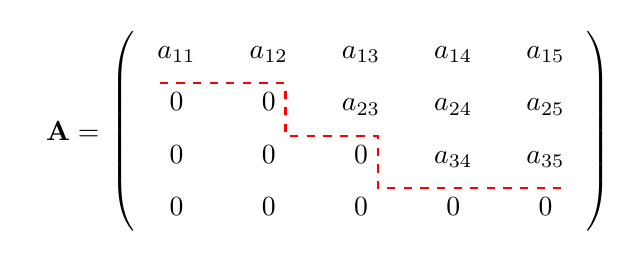
\begin{tikzpicture}
        \matrix (M) [matrix of math nodes]  { 
          \A = \\
        };
        \matrix(MM) [right=.1in of M, matrix of math nodes,nodes in empty cells,
          column sep=3ex,row sep=1ex,ampersand replacement=\&,left delimiter=(,right delimiter=)] {
          a_{11} \& a_{12} \& a_{13}  \& a_{14} \& a_{15}\\
          0 \& 0 \& a_{23}  \& a_{24} \& a_{25}\\
          0 \& 0 \& 0  \& a_{34} \& a_{35}\\
          0 \& 0 \& 0  \& 0 \& 0\\
        };
        \draw[thick,red,dashed] (MM-2-1.north west)--(MM-2-2.north east)
        --(MM-3-2.north east)--(MM-3-3.north east)
        --(MM-4-3.north east)--(MM-4-5.north east);
      \end{tikzpicture}
    \end{figure}
    其中$a_{11}\ne0, a_{23}\ne 0, a_{34}\ne 0$。
    \red{验证$\A$的行秩$=3$,列秩$=3$}。
  \end{footnotesize}
\end{frame}

\begin{frame}
  \begin{footnotesize}
    把$\A$按行和列分块为
    $$
    \A = \left(
    \begin{array}{c}
      \alphabd_1\\
      \alphabd_2\\
      \alphabd_3\\
      \alphabd_4
    \end{array}
    \right), \quad \B = (\betabd_1,\betabd_2,\betabd_3,\betabd_4,\betabd_5)
    $$
    下证$\alphabd_1,\alphabd_2,\alphabd_3$线性无关,$\betabd_1,\betabd_3,\betabd_4$线性无关。
          
  \end{footnotesize}
\end{frame}

\begin{frame}
  \begin{footnotesize}
    \begin{itemize}
    \item[(1)] 设
      $$
      x_1\alphabd_1+x_2\alphabd_2+x_3\alphabd_3=\zero,
      $$
      即
      $$
      x_1(a_{11},a_{12},a_{13},a_{14},a_{15})+
      x_2(0,0,a_{23},a_{24},a_{25})+
      x_3(0,0,0,a_{34},a_{35})=(0,0,0,0,0)
      $$ \pause 
      比较第一个分量
      $$
      x_1a_{11} = 0 \Rightarrow x_1=0.
      $$ \pause 从而
      $$
      x_2(0,0,a_{23},a_{24},a_{25})+
      x_3(0,0,0,a_{34},a_{35})=(0,0,0,0,0)
      $$ \pause 
      比较第3个分量
      $$
      x_2a_{23} = 0 \Rightarrow x_2=0.
      $$ \pause  从而
      $$
      x_3(0,0,0,a_{34},a_{35})=(0,0,0,0,0)
      $$\pause 
      同理得$x_3=0$。  于是$\alphabd_1,\alphabd_2,\alphabd_3$线性无关。 
      \pause \vspace{0.1in}

      又$\alphabd_4=\zero$,而零向量可由任何向量线性表示,这里
      $$
      \zero = 0\alphabd_1+0\alphabd_2+0\alphabd_3.
      $$
      故$\alphabd_1,\alphabd_2,\alphabd_3$是向量组$\alphabd_1,\alphabd_2,\alphabd_3,\alphabd_4$的极大无关组。所以矩阵$\A$的行秩为3。
    \end{itemize}
  \end{footnotesize}
\end{frame}


\begin{frame}
  \begin{footnotesize}
    \begin{itemize}
    \item[(2)] 设
      $$
      y_1\betabd_1 + y_3\betabd_3 + y_4\betabd_4=\zero
      $$
      即
      $$
      y_1\left(
      \begin{array}{c}
        a_{11}\\
        0\\
        0\\
        0
      \end{array}
      \right) + y_3\left(
      \begin{array}{c}
        a_{13}\\
        a_{23}\\
        0\\
        0
      \end{array}
      \right) + y_4\left(
      \begin{array}{c}
        a_{14}\\
        a_{24}\\
        a_{34}\\
        0
      \end{array}
      \right) = \left(
      \begin{array}{c}
        0\\
        0\\
        0\\
        0
      \end{array}
      \right)
      $$
      比较第三个分量得$y_4=0$。从而
      $$
      y_1\left(
      \begin{array}{c}
        a_{11}\\
        0\\
        0\\
        0
      \end{array}
      \right) + y_3\left(
      \begin{array}{c}
        a_{13}\\
        a_{23}\\
        0\\
        0
      \end{array}
      \right) = \left(
      \begin{array}{c}
        0\\
        0\\
        0\\
        0
      \end{array}
      \right)
      $$比较第二个分量得$y_3=0$。从而
      $$
      y_1\left(
      \begin{array}{c}
        a_{11}\\
        0\\
        0\\
        0
      \end{array}
      \right) = \left(
      \begin{array}{c}
        0\\
        0\\
        0\\
        0
      \end{array}
      \right)
      $$ 比较第一个分量得$y_1=0$。故$\betabd_1,\betabd_3,\betabd_4$线性无关。
    \end{itemize}
  \end{footnotesize}
\end{frame}

\begin{frame}
  \begin{footnotesize}
\begin{figure}
      \centering
      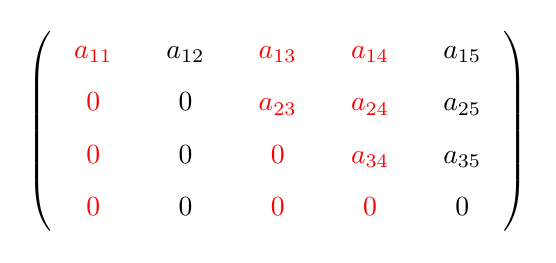
\begin{tikzpicture}
        \matrix(MM) [ matrix of math nodes,nodes in empty cells,
          column sep=3ex,row sep=1ex,ampersand replacement=\&,left delimiter=(,right delimiter=)] {
          \red{a_{11}} \& a_{12} \& \red{a_{13}}  \& \red{a_{14}} \& a_{15}\\
          \red{0} \& 0 \& \red{a_{23}}  \& \red{a_{24}} \& a_{25}\\
          \red{0} \& 0 \& \red{0}  \& \red{a_{34}} \& a_{35}\\
          \red{0} \& 0 \& \red{0}  \& \red{0} \& 0\\
        };
      \end{tikzpicture}
    \end{figure}
    
\pause 
    去掉向量组
    $$B:\betabd_1,\betabd_2,\betabd_3,\betabd_4,\betabd_5$$
    的最后一个分量,
    所得的新向量记为
    $$B^*:\betabd_1^*,\betabd_2^*,\betabd_3^*,\betabd_4^*,\betabd_5^*.$$
    注意去掉的分量全为$0$,故这两个向量组的相关性是一致的。
    \pause 
    \vspace{0.1in}
    
    由$\betabd_1,\betabd_3,\betabd_4$线性无关,
    则$\betabd_1^*,\betabd_3^*,\betabd_4^*$也线性无关。
    \pause 
    \vspace{0.1in}
    

    因任意$(3+1)=4$个$3$维向量必线性相关,
    故$\betabd_1^*,\betabd_3^*,\betabd_4^*$为向量组$B^*$的极大无关组,
    \pause 即向量组$B^*$中任何一个向量都可由$\betabd_1^*,\betabd_3^*,\betabd_4^*$线性表示,
    从而向量组$B$的任何一个向量都可以由$\betabd_1,\betabd_3,\betabd_4$线性表示。
    \pause 
    \vspace{0.1in}
    
    得证$\betabd_1,\betabd_3,\betabd_4$是向量组$B$的极大无关组,即矩阵$\A$的列秩为$3$。
  \end{footnotesize}
\end{frame}

\begin{frame}
  \begin{footnotesize}
    \begin{block}{结论}
      阶梯形矩阵的行秩等于列秩,其值等于阶梯形矩阵的非零行的行数。
    \end{block}
  \end{footnotesize}
\end{frame}


\begin{frame}
  \begin{footnotesize}
    \begin{block}{定理3.3.1}
      初等行变换不改变矩阵的行秩。
    \end{block}
    \pause
    \proofname
    只需证明每做一次对换、倍乘和倍加变换,矩阵的行秩不改变。    
    \pause\vspace{0.1in}

    设$\A$是$m\times n$矩阵,进行一次初等变换所得矩阵为$\B$。记$\A$的行向量为
    $$\red{A:~\alphabd_1,\alphabd_2,\cd,\alphabd_m.}$$ \pause     
    \begin{itemize}
    \item[(1)] 证明对换变换不改变矩阵的行秩。 \pause
      $$
      \A \xlongrightarrow[]{r_i\leftrightarrow r_j}\B
      $$
      因$\B$的行向量组
      $$\red{B:~\alphabd_1,\alphabd_2,\cd,\blue{c\alphabd_j},,\cd,\blue{c\alphabd_i},\cd,\alphabd_m}$$
      与$\A$的行向量组$$\red{B:~\alphabd_1,\alphabd_2,\cd,\blue{c\alphabd_i},,\cd,\blue{c\alphabd_j},\cd,\alphabd_m}$$
      一致,故$\B$的行秩等于$\A$的行秩。 \\[0.1in] \pause
    \end{itemize}
  \end{footnotesize}
\end{frame}


\begin{frame}
  \begin{footnotesize}
    \begin{itemize}
    \item[(2)] 证明倍乘变换不改变矩阵的行秩。 \pause
      $$
      \A \xlongrightarrow[]{r_i\times c }\B,
      $$
      其中$c\ne 0$。因$\B$的行向量组
      $$\red{B:~\alphabd_1,\alphabd_2,\cd,\blue{c\alphabd_i},\cd,\alphabd_m}$$
      与$\A$的行向量组
      $$\red{A:~\alphabd_1,\alphabd_2,\cd,\blue{\alphabd_i},\cd,\alphabd_m}$$
      等价,故$\B$的行秩等于$\A$的行秩。
    \end{itemize}
  \end{footnotesize}
\end{frame}

\begin{frame}
  \begin{footnotesize}
    \begin{itemize}
    \item[(3)] 证明倍乘变换不改变矩阵的行秩。 \pause
      $$
      \A \xlongrightarrow[]{r_i+ r_j \times c  }\B,
      $$
      因$\B$的行向量组
      $$B:~\alphabd_1,\alphabd_2,\cd,\red{\alphabd_i+c\alphabd_j},\cd,\alphabd_m$$
      与$\A$的行向量组
      $$\red{A:~\alphabd_1,\alphabd_2,\cd,\blue{\alphabd_i},\cd,\alphabd_m}$$
      等价,故$\B$的行秩等于$\A$的行秩。
    \end{itemize}
  \end{footnotesize}
\end{frame}

\begin{frame}
  \begin{footnotesize}
    \begin{block}{定理3.3.2}
      初等行变换不改变矩阵的列秩。
    \end{block}
    \pause
    \proofname
    设
    $$
    \A = (\alphabd_1,\alphabd_2,\cd,\alphabd_m) \xlongrightarrow[]{\mbox{初等行变换}}
    (\betabd_1,\betabd_2,\cd,\betabd_m) = \B
    $$ \pause
    在$\A,\B$中相同位置任取某$s$个列向量:
    $$
    \alphabd_{i_1},\alphabd_{i_2},\cd,\alphabd_{i_s} \mbox{~~和~~}
    \betabd_{i_1},\betabd_{i_2},\cd,\betabd_{i_s},
    $$
    分别记为向量组$A^*$和$B^*$。\pause设
    \begin{eqnarray}
      x_1\alphabd_{i_1}+x_2\alphabd_{i_2}+\cd+x_s\alphabd_{i_s} =\zero, \label{thm3.3.2-1}\\[0.1in]
      x_1\betabd_{i_1}+x_2\betabd_{i_2}+\cd+x_s\betabd_{i_s} =\zero, \label{thm3.3.2-2}
    \end{eqnarray} \pause
    注意到方程组(\ref{thm3.3.2-2})是方程组(\ref{thm3.3.2-1})经过高斯消元法得到,故两方程组同解。\pause 即向量组$A^*$和$B^*$有完全相同的线性关系。得证$\A,\B$列秩相等。
    \pause
    \begin{block}{注}
      定理3.3.2提供了求向量组的秩与极大无关组的一种简便而有效的方法。
    \end{block}
  \end{footnotesize}
\end{frame}

\begin{frame}
  \begin{footnotesize}
    \begin{exampleblock}{例1}
      设向量组
      $$
      \alphabd_1=\left(
      \begin{array}{r}
        -1\\-1\\0\\0
      \end{array}
      \right),~~ \alphabd_2=\left(
      \begin{array}{r}
        1\\2\\1\\-1
      \end{array}
      \right),~~ \alphabd_3=\left(
      \begin{array}{r}
        0\\1\\1\\-1
      \end{array}
      \right),~~ \alphabd_4=\left(
      \begin{array}{r}
        1\\3\\2\\1
      \end{array}
      \right),~~ \alphabd_5=\left(
      \begin{array}{r}
        2\\6\\4\\-1
      \end{array}
      \right)
      $$
      求向量组的秩及其一个极大无关组,并将其余向量用该极大无关组线性表示。
    \end{exampleblock}
    \pause\jiename
    作矩阵$\A=(\alphabd_1,\alphabd_2,\alphabd_3,\alphabd_4,\alphabd_5)$,由
    $$
    \begin{array}{rl}
    \A &= \left(
    \begin{array}{rrrrr}
      -1&1&0&1&2\\
      -1&2&1&3&6\\
      0&1&1&2&4\\
      0&-1&-1&1&-1
    \end{array}
    \right) \xlongrightarrow[r_2+r_1]{ r_1\times(-1)}
    \left(
    \begin{array}{rrrrr}
      1&-1&0&-1&-2\\
      0&1&1&2&4\\
      0&1&1&2&4\\
      0&-1&-1&1&-1
    \end{array}
    \right)\\[0.4in]
    &\xlongrightarrow[r_4+r_2]{r_3- r_2}
    \left(
    \begin{array}{rrrrr}
      1&-1&0&-1&-2\\
      0&1&1&2&4\\
      0&0&0&0&0\\
      0&0&0&3&3
    \end{array}
    \right) \xlongrightarrow[r_3\leftrightarrow r_4]{r_4\div 3}
    \left(
    \begin{array}{rrrrr}
      1&-1&0&-1&-2\\
      0&1&1&2&4\\
      0&0&0&1&1\\
      0&0&0&0&0
    \end{array}
    \right)
    \end{array}
    $$
  \end{footnotesize}
\end{frame}

\begin{frame}
  \begin{footnotesize}
    $$
    \begin{array}{rl}
      & \xlongrightarrow[r_2 -2 r_3]{r_1+r_3}
    \left(
    \begin{array}{rrrrr}
      1&-1&0&0&-1\\
      0&1&1&0&2\\
      0&0&0&1&1\\
      0&0&0&0&0
    \end{array}
    \right) \xlongrightarrow[]{r_1+r_2}
    \left(
    \begin{array}{rrrrr}
      1&0&1&0&1\\
      0&1&1&0&2\\
      0&0&0&1&1\\
      0&0&0&0&0
    \end{array}
    \right) = \B
    \end{array}
    $$
    将最后一个阶梯矩阵$\B$记为$(\betabd_1,\betabd_2,\betabd_3,\betabd_4,\betabd_5)$
    \pause 
    \vspace{0.1in}

    易知$\betabd_1,\betabd_2,\betabd_4$为$\B$的列向量组的一个极大无关组,故$\alphabd_1,\alphabd_2,\alphabd_4$也为$\A$的列向量组的一个极大无关组,故
    $$
    \rr(\alphabd_1,\alphabd_2,\alphabd_3,\alphabd_4,\alphabd_5)=3,
    $$
    且
    $$
    \begin{array}{l}
      \alphabd_3=\alphabd_1+\alphabd_2,\\
      \alphabd_5=\alphabd_1+2\alphabd_2+\alphabd_4,\\
    \end{array}
    $$
    
  \end{footnotesize}
\end{frame}

\begin{frame}
  \begin{footnotesize}
    由定理3.3.1与定理3.3.2可以推出:
    \purple{初等列变换也不改变矩阵的列秩与行秩。}
    \pause
    \begin{block}{定理3.3.3}
      初等变换不改变矩阵的行秩与列秩。
    \end{block}

    \pause
    \begin{block}{定理3.3.4}
      矩阵的行秩等于其列秩。
    \end{block}
    \pause \proofname
    对$\A$做初等行变换得到阶梯矩阵$\U$,则有
    $$
    \begin{array}{rl}
      \A\mbox{的行秩}&=\U\mbox{的行秩}\\[0.1in]
      &=\U\mbox{的列秩}=\A\mbox{的列秩}
    \end{array}
    $$

  \end{footnotesize}
\end{frame}

\begin{frame}
  \begin{footnotesize}
    \begin{block}{定义(矩阵的秩)}
      矩阵的行秩或列秩的数值,称为\red{矩阵的秩}。记作
      $$
      \rr(\A)  \quad \mbox{或} \quad 
      \mathrm{R} (\A)  \quad \mbox{或} \quad
      \mathrm{rank} (\A)
      $$
    \end{block}
    \pause 
    \begin{block}{定义(满秩矩阵)}
      对于$n$阶方阵,若
      $$
      \rr(\A) = n,
      $$
      则称$\A$为\red{满秩矩阵}。
    \end{block}
  \end{footnotesize}
\end{frame}

\begin{frame}
  \begin{footnotesize}
    \begin{block}{定理3.3.5}
      对于$n$阶方阵,下列表述等价:
      \begin{itemize}
      \item[(1)] $\A$为满秩矩阵。
      \item[(2)] $\A$为可逆矩阵。
      \item[(3)] $\A$为非奇异矩阵。
      \item[(4)] $\A\ne 0$。
      \end{itemize}
    \end{block}
    \pause\proofname
    只需证明前两个表述等价。 \pause

    \begin{itemize}
    \item [\red{(1)$\Rightarrow$(2)}]    
      设$\rr(\A)=n$,记$\A$的行简化阶梯形矩阵为$\B$,则$\B$有$n$个非零行,\pause 由行简化阶梯形矩阵的结构知
    $
    \B=\II,
    $ \pause
    即存在可逆矩阵$\PP$使得
    $$
    \PP\A=\II,
    $$
    故$\A^{-1}=\PP$,即$\A$可逆。\pause
  \item [\red{(2)$\Rightarrow$(1)}]   
    若$\A$可逆,记$\A^{-1}=\PP_0$,则
    $$
    \PP_0\A=\II,
    $$ \pause
    即$\A$经过初等行变换可以得到$\II$,故$\rr(\A)=\rr(\II)=n$。
    \end{itemize}
  \end{footnotesize}
\end{frame}

\begin{frame}
  \begin{footnotesize}
    \begin{block}{子式与主子式}
      对矩阵$\A=(a_{ij})_{m\times n}$,任意挑选$k$行($i_1,i_2,\cd,i_k$行)与$k$列($j_1,j_2,\cd,j_k$列),
      其交点上的$k^2$个元素按原顺序排成的$k$阶行列式
      \begin{equation}\label{subdet}
        \left|
        \begin{array}{cccc}
          a_{i_1j_1} & a_{i_1j_2} & \cd & a_{i_1j_k}\\
          a_{i_2j_1} & a_{i_2j_2} & \cd & a_{i_2j_k}\\
          \vd & \vd && \vd\\
          a_{i_kj_1} & a_{i_kj_2} & \cd & a_{i_kj_k}\\
        \end{array}
        \right|
      \end{equation}
      称为$\A$的\red{$k$阶子行列式},简称$\A$的\red{$k$阶子式}。\pause 
      \begin{itemize}
      \item 当(\ref{subdet})等于零时,称为\red{$k$阶零子式};
      \item 当(\ref{subdet})不等于零时,称为\red{$k$阶非零子式};
      \item 当(\ref{subdet})的$j_1=i_1,~j_2=i_2,~\cd,~j_k=i_k$,称为$\A$的\red{$k$阶主子式}。
      \end{itemize}
    \end{block}
  \end{footnotesize}
\end{frame}

\begin{frame}
  \begin{footnotesize}
    \begin{block}{注}
      若$\A$存在$r$阶非零子式,而所有$r+1$阶子式(如果有)都等于零,则矩阵$\A$的非零子式的最高阶数为$r$。
    \end{block}
    \pause
    事实上,由行列式的按行展开可知,若所有$r+1$阶子式都等于零,可得到所有更高阶的子式都等于零。
  \end{footnotesize}
\end{frame}

\begin{frame}
  \begin{footnotesize}
    \begin{block}{定理3.3.6}
      $\rr(\A)=r$的充分必要条件是$\A$的非零子式的最高阶数为$r$。
    \end{block}
    \pause
    \proofname
    \begin{itemize}
    \item[$(\Rightarrow)$] 设$\rr(\A)=r$,即$\A$的行秩为$r$,不妨设$\A$的前$r$行构成的矩阵$\A_1$的行秩为$r$,
      其列秩也为$r$;不妨设$\A_1$的前$r$个列向量线性无关。\vspace{0.05in} \pause 

      由定理3.3.5可知,$\A$的左上角$r$阶子式为非零子式。\vspace{0.05in} \pause 

      又因为$\A$的任意$r+1$个行向量线性相关,所以$\A$的任意$r+1$阶子式都是零子式(\purple{因为其中有一行可由其余$r$行线性表示}),
      因此$\A$的非零子式的最高阶数为$r$。 \vspace{0.05in} \pause 

    \item[$(\Leftarrow)$] 
      不妨设$\A$的左上角$r$阶子式$|\A_r|\ne 0$,于是$\A_r$可逆,其$r$个行向量线性无关。\pause
      将它们添加分量称为$\A$的前$r$个行向量,它们也线性无关。\vspace{0.05in} \pause 

      而$\A$的任何$r+1$个行向量必线性相关(\purple{否则,$\A$中存在$r+1$阶非零子式,这与题设矛盾}),故$\A\mbox{的行秩}=\rr(\A)=r$.
    \end{itemize}
  \end{footnotesize}
\end{frame}


\begin{frame}
  \begin{footnotesize}
    \begin{block}{关于矩阵的秩的基本结论}
      \begin{itemize}
      \item[(1)]  $\red{\rr(\A)=\A\mbox{的行秩}=\A\mbox{的列秩}=\A\mbox{的非零子式的最高阶数}}$
      \item[(2)]  \red{初等变换不改变矩阵的秩}
      \end{itemize}
    \end{block}
  \end{footnotesize}
\end{frame}


\begin{frame}
  \begin{footnotesize}
    \begin{block}{性质1}
      $$
      \red{\max\{\rr(\A),~\rr(\B)\}~~\le~~ \rr(\A,~\B) ~~\le~~ \rr(\A) + \rr(\B).}
      $$
      特别地,当$\B=\bb$为非零向量时,有
      $$
      \red{\rr(\A)~~\le~~\rr(\A,~\bb)~~\le~~\rr(\A)+1.}
      $$
    \end{block}
    \pause
    $$
    \rr(\A,\bb) = \left\{
    \begin{array}{ll}
      \rr(\A) & \Longleftrightarrow~~ \bb\mbox{可以被}\A\mbox{的列向量线性表示}\\[0.1in]
      \rr(\A)+1 & \Longleftrightarrow~~ \bb\mbox{不能被}\A\mbox{的列向量线性表示}
    \end{array}
    \right.
    $$
  \end{footnotesize}
\end{frame}

\begin{frame}
  \begin{footnotesize}
    设$$\A=\left(
    \begin{array}{cc}
      1&0\\
      0&1\\
      0&0
    \end{array}
    \right),$$
    \begin{itemize}
    \item[(1)] 取$\bb=\left(
    \begin{array}{cc}
      1\\
      2\\
      0
    \end{array}
    \right)$,则
    $$
    (\A,~\bb) = \left(
    \begin{array}{ccc}
      1&0&\red{1}\\
      0&1&\red{2}\\
      0&0&\red{0}
    \end{array}
    \right) \xlongrightarrow[]{c_3-(c_1+2c_2)}
    \left(
    \begin{array}{ccc}
      1&0&\red{0}\\
      0&1&\red{0}\\
      0&0&\red{0}
    \end{array}
    \right) = (\A, \zero),
    $$
    故$\rr(\A,\bb)=\rr(\A,\zero)=\rr(\A)$。\\[0.1in] \pause 
  \item[(2)] 取$\bb=\left(
    \begin{array}{cc}
      0\\
      0\\
      1
    \end{array}
    \right)$,则
    $$
    (\A,~\bb) = \left(
    \begin{array}{ccc}
      1&0&\red{0}\\
      0&1&\red{0}\\
      0&0&\red{1}
    \end{array}
    \right),
    $$
    $\bb$不能由$\A$的列向量线性表示,故
    $\rr(\A,\bb)=\rr(\A)+1.$
    \end{itemize}
    
  \end{footnotesize}
\end{frame}


\begin{frame}
  \begin{footnotesize}
    \proofname
    \begin{itemize}
    \item
      因为$\A$的列均可由$(\A,\B)$的列线性表示,故
      $$
      \rr(\A) \le \rr(\A,\B),
      $$ \pause 
      同理
      $$
      \rr(\B) \le \rr(\A,\B),
      $$\pause 
      所以
      $$
      \max\{\rr(\A),~\rr(\B)\} \le \rr(\A,\B),
      $$ \\[0.1in]
    \item \pause 
      设$\rr(\A)=p, ~\rr(\B)=q$,%将$\A,\B$按列分块为
    %% $$
    %% \A=(\alphabd_1,~\cd,~\alphabd_n), ~~
    %% \B=(\betabd_1,~\cd,~\betabd_n).
    %% $$ \pause 
    $\A$和$\B$的列向量组的极大无关组分别为
    $$
    \alphabd_1,~\cd,~\alphabd_p \mbox{~~和~~}
    \betabd_1,~\cd,~\betabd_q. \pause 
    $$ \pause 
    显然$(\A,~\B)$的列向量组可由向量组$\alphabd_1,~\cd,~\alphabd_p,~
    \betabd_1,~\cd,~\betabd_q$线性表示,故
    $$
    \rr(\A,~\B) = (\A,~\B)\mbox{的列秩} \le \rr(\alphabd_1,~\cd,~\alphabd_p,~
    \betabd_1,~\cd,~\betabd_q) \le p+q.
    $$
    \end{itemize}
  \end{footnotesize}
\end{frame}


\begin{frame}
  \begin{footnotesize}
    \begin{block}{注}
      \begin{itemize}
      \item 不等式
        $$
        \min\{\rr(\A),~\rr(\B)\} ~~\le~~ \rr(\A,~\B)
        $$
        意味着:在$\A$的右侧添加新的列,只有可能使得秩在原来的基础上得到增加;当$\B$的列向量能被$\A$的列向量线性表示时,等号成立。\\[0.1in]\pause 
      \item 不等式
        $$
        \rr(\A,~\B) ~~\le~~ \rr(\A)+\rr(\B)
        $$
        意味着:对$(\A,~\B)$,有可能$\A$的列向量与$\B$的列向量出现线性相关,合并为$(\A,~\B)$的秩一般会比$\rr(\A)+\rr(\B)$要小。
      \end{itemize}
    \end{block}
  \end{footnotesize}
\end{frame}




\begin{frame}
  \begin{footnotesize}
     \begin{block}{性质2}
      $$
      \red{\rr(\A+\B) \le \rr(\A)+\rr(\B).}
      $$
    \end{block}
    \pause\proofname
    设$\rr(\A)=p, ~\rr(\B)=q$,
    $\A$和$\B$的列向量组的极大无关组分别为
    $$
    \alphabd_1,~\cd,~\alphabd_p \mbox{~~和~~}
    \betabd_1,~\cd,~\betabd_q. \pause 
    $$ \pause 
    显然$\A+\B$的列向量组可由向量组$\alphabd_1,~\cd,~\alphabd_p,~
    \betabd_1,~\cd,~\betabd_q$线性表示,故
    $$
    \rr(\A+\B) = \A+\B\mbox{的列秩} \le \rr(\alphabd_1,~\cd,~\alphabd_p,~
    \betabd_1,~\cd,~\betabd_q) \le p+q.
    $$
    \pause 
    \begin{block}{注}
      将矩阵$\A$和$\B$合并、相加,只可能使得秩减小。
    \end{block}
  \end{footnotesize}
\end{frame}




\begin{frame}
  \begin{footnotesize}
    \begin{block}{性质3}
      $$
      \red{\rr(\A\B) \le \min(\rr(\A),~\rr(\B)).}
      $$
    \end{block}
    \pause
    \proofname
    设$\A,\B$分别为$m\times n, n\times s$矩阵,将$\A$按列分块,则
    $$
    \A\B = (\alphabd_1,~\cd,~\alphabd_n) \left(
    \begin{array}{cccc}
      b_{11}&b_{12}&\cd&b_{1s}\\
      b_{21}&b_{22}&\cd&b_{2s}\\
      \vd&\vd&&\vd\\
      b_{n1}&b_{n2}&\cd&b_{ns}
    \end{array}
    \right).
    $$ \pause 
    由此可知,$\A\B$的列向量组可由$\alphabd_1,~\alphabd_2,~\cd,~\alphabd_n$线性表示,故
    $$
    \rr(\A\B) = \A\B\mbox{的列秩} \le \A\mbox{的列秩} = \rr(\A).
    $$
    \pause
    类似地,将$\B$按行分块,可得$$\rr(\A\B)\le \rr(\B).$$
      \end{footnotesize}
\end{frame}


\begin{frame}
  \begin{footnotesize}
    该定理告诉我们,
    \begin{block}{}
      对一个向量组进行线性组合,可能会使向量组的秩减小。
    \end{block}
  \end{footnotesize}
\end{frame}


\begin{frame}
  \begin{footnotesize}
    \begin{block}{性质4}
      设$\A$为$m\times n$矩阵,$\PP,\QQ$分别为$m$阶、$n$阶可逆矩阵,则
      $$
      \rr(\A) = \rr(\PP\A) = \rr(\A\QQ)  = \rr(\PP\A\QQ).
      $$
    \end{block}
    \pause\proofname
    \begin{itemize}
    \item[方法一] 
      可逆矩阵$\PP,~\QQ$可表示为若干个初等矩阵的乘积,而初等变换不改变矩阵的秩,故结论成立。 \pause
    \item[方法二]
      因
      $$
      \rr(\A) = \rr(\PP^{-1}(\PP\A)) \le \rr(\PP\A) \le \rr(\A)
      $$
      故
      $$
      \rr(\A) = \rr(\PP\A).
      $$
      \pause 
      同理可证其他等式。
    \end{itemize}
  \end{footnotesize}
\end{frame}


\begin{frame}
  \begin{footnotesize}
    \begin{exampleblock}{例3.3.2}
      设$\A$是$m\times n$矩阵,且$m<n$,证明:$|\A^T\A|=0$.
    \end{exampleblock}
    \pause
    \jiename
    由于$\rr(\A)=\rr(\A^T)\le \min\{m,n\}<n$,根据性质2,有
    $$
    \rr(\A^T\A) \le \min\{\rr(\A^T),~\rr(\A)\} < n,
    $$
    而$\A^T\A$为$n$阶矩阵,故$|\A^T\A|=0$。
  \end{footnotesize}
\end{frame}


\begin{frame}
  \begin{footnotesize}
    \begin{block}{矩阵的相抵}
      若矩阵$\A$经过初等变换化为$\B$(\purple{亦即存在可逆矩阵$\PP$和$\QQ$使得$\PP\A\QQ=\B$}),就称$\A$\red{相抵于}$\B$,记作$\A\cong\B$
    \end{block}
    \pause
    \begin{block}{相抵关系的性质}
      \begin{itemize}
      \item 反身性
        $$
        \A\cong\A
        $$
      \item 对称性
        $$
        \A\cong\B ~~\Rightarrow~~ \B\cong\A
        $$
      \item 传递性
        $$
        \A\cong\B,~~\B\cong\C ~~\Rightarrow~~ \A\cong\C
        $$
      \end{itemize}
    \end{block}
    
  \end{footnotesize}
\end{frame}


\begin{frame}
  \begin{footnotesize}
    \begin{block}{阶梯形矩阵}
      若矩阵$\A$满足
      \begin{itemize}
      \item[(1)] 零行在最下方;
      \item[(2)] 非零行首元的列标号随行标号的增加而严格递增,
      \end{itemize}
      则称$\A$为\red{阶梯形矩阵}。
    \end{block}
    \pause
    \begin{exampleblock}{例}
      $$
      \left(
      \begin{array}{rrrr}
        2&0&2&1\\
        0&5&2&-2\\
        0&0&3&2\\
        0&0&0&0
      \end{array}
      \right)
      $$
    \end{exampleblock}
  \end{footnotesize}
\end{frame}


\begin{frame}
  \begin{footnotesize}
    \begin{block}{阶梯形矩阵}
      若矩阵$\A$满足
      \begin{itemize}
      \item[(1)] 它是阶梯形矩阵;
      \item[(2)] 非零行首元所在的列除了非零行首元外,其余元素全为零,
      \end{itemize}
      则称$\A$为\red{行简化阶梯形矩阵}。
    \end{block}
    \pause
    \begin{exampleblock}{例}
      $$
      \left(
      \begin{array}{rrrr}
        2&0&0&1\\
        0&5&0&-2\\
        0&0&3&2\\
        0&0&0&0
      \end{array}
      \right)
      $$
    \end{exampleblock}
  \end{footnotesize}
\end{frame}

\begin{frame}
  \begin{footnotesize}
    \begin{block}{定理3.3.7}
      若$\A$为$m\times n$矩阵,且$\rr(\A)=r$,则一定存在可逆的$m$阶矩阵$\PP$和$n$阶矩阵$\QQ$使得
      $$
      \PP\A\QQ=\left(
      \begin{array}{cc}
        \II_r&\zero\\
        \zero&\zero
      \end{array}
      \right)_{m\times n} = \U.
      $$
    \end{block}
    \pause \proofname
    对$\A$做初等行变换,可将$\A$化为有$r$个非零行的行简化阶梯形矩阵,即存在初等矩阵$\PP_1,\PP_2,\cd,\PP_s$使得
    $$
    \PP_s\cd\PP_2\PP_1\A=\U_1.
    $$
    \pause
    对$\U_1$做初等列变换可将$\U_1$化为$\U$,即存在初等矩阵$\QQ_1,\QQ_2,\cd,\QQ_t$使得
    $$
    \U_1\QQ_1\QQ_2\cd\QQ_t=\U
    $$
    \pause
    记
    $$
    \purple{\PP_s\cd\PP_2\PP_1=\PP, ~~\QQ_1\QQ_2\cd\QQ_t=\QQ,}
    $$
    则有
    $$
    \PP\A\QQ=\U.
    $$
  \end{footnotesize}
\end{frame}

\begin{frame}
  \begin{footnotesize}
    \begin{block}{定义(相抵标准形)}
      设$\rr(\A_{m\times n})=r$,则矩阵
      $$
      \left(
      \begin{array}{cc}
        \II_r&\zero\\
        \zero&\zero
      \end{array}
      \right)_{m\times n} 
      $$称为$\A$的\blue{相抵标准形},简称\blue{标准形}。
    \end{block}
    \pause 
    \begin{block}{注}
      \begin{itemize}
      \item 秩相等的同型矩阵,必有相同的标准形。\\[0.1in]
      \item 两个秩相等的同型矩阵是相抵的。
      \end{itemize}
    \end{block}
  \end{footnotesize}
\end{frame}

\begin{frame}
  \begin{footnotesize}
    \begin{exampleblock}{例3}
      设$\A$为$m\times n$矩阵($m>n$),$\rr(\A)=n$,证明:存在$n\times m$矩阵$\B$使得
      $$
      \B\A=\II_n.
      $$
    \end{exampleblock}
    \pause
    \proofname
    由定理3.3.7可知,存在$m$阶可逆矩阵$\PP$与$n$阶可逆矩阵$\QQ$使得
    $$
    \PP\A\QQ=\left(
    \begin{array}{c}
      \II_n\\
      \zero_1
    \end{array}
    \right) \pause    
    ~~~\Rightarrow~~~
    \PP\A=\left(
    \begin{array}{c}
      \II_n\\
      \zero_1
    \end{array}
    \right)\QQ^{-1}=\left(
    \begin{array}{c}
      \QQ^{-1}\\
      \zero_1
    \end{array}
    \right)
    $$
    其中$\zero_1$为$(m-n)\times n$零矩阵。 \pause
    
    取
    $$
    \C=(\QQ~~\zero_2),
    $$
    其中$\zero_2$为$n\times(m-n)$阶零矩阵,\pause 则
    $$
    \C\PP\A=(\QQ~~\zero_2)\left(
    \begin{array}{c}
      \QQ^{-1}\\
      \zero_1
    \end{array}
    \right)=\QQ\QQ^{-1}+\zero_2\zero_1=\II_n.
    $$\pause 
    故存在$\B=\C\PP$使得
    $$
    \B\A=\II_n.
    $$
  \end{footnotesize}
\end{frame}


\begin{frame}
  \begin{footnotesize}
    \begin{exampleblock}{例4}
      设$\alphabd_1=(1,3,1,2), ~\alphabd_2=(2,5,3,3), ~\alphabd_3=(0,1,-1,a), ~\alphabd_4=(3,10,k,4)$,
      试求向量组$\alphabd_1,~\alphabd_2,~\alphabd_3,~\alphabd_4$的秩,并将$\alphabd_4$用$\alphabd_1,~\alphabd_2,~\alphabd_3$线性表示。
    \end{exampleblock}
    \pause \jiename
    将4个向量按列排成一个矩阵$\A$,对$\A$进行初等变换,将其化为阶梯形矩阵$\U$,即
    $$
    \A=\left(
    \begin{array}{rrrr}
    1&2&0&3\\
    3&5&1&10\\
    1&3&-1&k\\
    2&3&a&4
    \end{array}
    \right) \xlongrightarrow[]{\mbox{初等行变换}}
    \left(
    \begin{array}{rrcc}
    1&2&0&3\\
    0&-1&1&1\\
    0&0&a-1&-3\\
    0&0&0&k-2
    \end{array}
    \right)
    $$
    \pause 
    \begin{itemize}
    \item[(1)] 当$a=1$或$k=2$时,$\U$只有3个非零行,故
      $$\rr(\alphabd_1,\alphabd_2,\alphabd_3,\alphabd_4)=\rr(\A)=3. $$ 
    \item[(2)] \pause 当$a\ne1$且$k\ne2$时,
      $$\rr(\alphabd_1,\alphabd_2,\alphabd_3,\alphabd_4)=\rr(\A)=4.$$
    \end{itemize}
      \end{footnotesize}
\end{frame}


\begin{frame}
  \begin{footnotesize}
    $$
    \A=\left(
    \begin{array}{rrrr}
      1&2&0&3\\
      3&5&1&10\\
      1&3&-1&k\\
      2&3&a&4
    \end{array}
    \right) \xlongrightarrow[]{\mbox{初等行变换}}
    \left(
    \begin{array}{rrcc}
      1&2&0&3\\
      0&-1&1&1\\
      0&0&a-1&-3\\
      0&0&0&k-2
    \end{array}
    \right)
    $$
    \begin{itemize}
    \item 当$k=2$且$a\ne1$时,$\alphabd_4$可由$\alphabd_1,~\alphabd_2,~\alphabd_3$线性表示,
      且
      $$
      \alphabd_4=-\frac{1+5a}{1-a}\alphabd_1+\frac{2+a}{1-a}\alphabd_2+\frac{3}{1-a}\alphabd_3.
      $$
    \item \pause 当$k\ne2$或$a=1$时,$\alphabd_4$不能由$\alphabd_1,~\alphabd_2,~\alphabd_3$线性表示。
    \end{itemize}
  \end{footnotesize}
\end{frame}


\begin{frame}
  \begin{footnotesize}
    \begin{exampleblock}{例5}
      设
      $$
      \A=\left(
      \begin{array}{rrr}
        1&2&1\\
        2&2&-2\\
        -1&t&5\\
        1&0&-3
      \end{array}
      \right)
      $$
      已知$\rr(\A)=2$,求$t$。
    \end{exampleblock}
    \pause
    \jiename
    $$
    \A \xlongrightarrow[]{\mbox{初等行变换}} \left(
    \begin{array}{ccr}
      1&2&1\\
      0&-2&-4\\
      0&2+t&6\\
      0&0&0
    \end{array}
    \right)=\B
    $$ \pause
    由于$\rr(\B)=\rr(\A)$,故$\B$中第2、3行必须成比例,即
    $$
    \frac{-2}{2+t}=\frac{-4}6,
    $$
    即得$t=1$。
  \end{footnotesize}
\end{frame}

%% \begin{frame}
%%   \begin{footnotesize}
%%     \begin{exampleblock}{例6}
%%       已知$\rr(\B)=2$,
%%       $$
%%       \A=\left(
%%       \begin{array}{ccc}
%%         1&2&0\\
%%         0&a&1\\
%%         1&3&b
%%       \end{array}
%%       \right).
%%       $$
%%       问
%%       \begin{itemize}
%%       \item[(1)] $a,b$满足什么条件时,$\rr(\A\B)=2$;
%%       \item[(2)] $\A$与$\B$满足什么条件时,$\rr(\A\B)=1$。
%%       \end{itemize}
%%     \end{exampleblock}
%%     \jiename\pause
%%     \begin{itemize}
%%     \item[(1)] 当$\A$可逆时,$\rr(\A\B)=\rr(\B)=2$。此时,
%%       $$
%%       |\A| = ab-1\ne 0.
%%       $$
%%     \item[(2)]\pause 当$ab-1=0$时,$\A$不可逆,且$\rr(\A)=2$。\pause
%%       $\A$的列向量组线性相关,故$\A\xx=\zero$有非零解。
%%     \end{itemize}
%%   \end{footnotesize}
%% \end{frame}

%% \begin{frame}
%%   \begin{footnotesize}
    
%%   \end{footnotesize}
%% \end{frame}


%% \begin{frame}
%%   \begin{footnotesize}
    
%%   \end{footnotesize}
%% \end{frame}


%% \begin{frame}
%%   \begin{footnotesize}
    
%%   \end{footnotesize}
%% \end{frame}

%% \begin{frame}
%%   \begin{footnotesize}
    
%%   \end{footnotesize}
%% \end{frame}

%% \begin{frame}
%%   \begin{footnotesize}
    
%%   \end{footnotesize}
%% \end{frame}

  % \section{齐次线性方程组有非零解的条件及解的结构}

\begin{frame}
  \begin{footnotesize}
    设$\mathbf A$为$m\times n$矩阵,考察以$\A$为系数矩阵的齐次线性方程组
    \begin{equation}\label{ax0}
      \A\xx=\zero.
    \end{equation}    
    \pause
    若将$\A$按列分块为
    $$
    \A = (\alphabd_1,~\alphabd_2,~\cd,~\alphabd_n),
    $$
    齐次方程组(\ref{ax0})可表示为
    $$
    x_1\alphabd_1+x_2\alphabd_2+\cd+x_n\alphabd_n=\zero.
    $$
    \pause
    齐次方程组(\ref{ax0})有\blue{非零解}的充分必要条件是$\alphabd_1,~\alphabd_2,~\cd,~\alphabd_n$\blue{线性相关},即
    $$
    \RR(\A) = \RR(\alphabd_1,~\alphabd_2,~\cd,~\alphabd_n) < n.
    $$
  \end{footnotesize}
\end{frame}

\begin{frame}
  \begin{footnotesize}
    \begin{block}{定理3.4.1}
      设$\A$为$m\times n$矩阵,则
      $$
      \blue{\underline{\A\xx=\zero\mbox{有非零解}}} ~~\Longleftrightarrow~~
      \blue{\underline{\RR(\A)<n}}.$$
    \end{block}
  \end{footnotesize}
\end{frame}

\begin{frame}
  \begin{footnotesize}
    \begin{block}{定理3.4.1的等价命题}
      设$\A$为$m\times n$矩阵,则
      $$
      \blue{\underline{\A\xx=\zero\mbox{只有零解}}} ~~\Longleftrightarrow~~
      \blue{\underline{\RR(\A)=n=\A\mbox{的列数}}}.
      $$
    \end{block}
  \end{footnotesize}
\end{frame}

\begin{frame}
  \begin{footnotesize}
    \begin{exampleblock}{例1}
      设$\A$为$n$阶矩阵,证明:存在$n\times s$矩阵$\B\ne \zero$,使得$\A\B=\zero$的充分必要条件是
      $$
      |\A|=0.
      $$      
    \end{exampleblock}
    \pause
    \proofname
    $|\A|=0~~\Longleftrightarrow~~\A\xx=\zero$有非零解。\pause 下证
    $$
    \purple{\mbox{存在}n\times s\mbox{矩阵}\B\ne 0\mbox{使得}\A\B=\zero
      ~~\Longleftrightarrow~~\A\xx=\zero\mbox{有非零解}}.
    $$     \pause
    \begin{itemize}
    \item[($\red{\Longrightarrow}$)]
      设$\A\B=\zero$,则$\B$的解向量为$\A\xx=\zero$的解。又$\B\ne\zero$,则$\B$至少有一个非零列向量,
      从而$\A\xx=\zero$至少有一个非零解。\\[0.2in] \pause 
    \item[($\red{\Longleftarrow}$)]
      设$\A\xx=\zero$有非零解,任取一个非零解$\betabd$,令
      $$
      \B=(\betabd,~\zero,~\cd,~\zero)
      $$
      则$\B\ne\zero$,且$\A\B=\zero$。
    \end{itemize}

  \end{footnotesize}
\end{frame}

\begin{frame}
  \begin{footnotesize}
    \begin{block}{定理3.4.2}
      若$\xx_1,~\xx_2$为齐次线性方程组$\A\xx=\zero$的两个解,则
      $$
      k_1\xx_1+k_2\xx_2\quad(k_1,~k_2\mbox{为任意常数})
      $$
      也是它的解。
    \end{block}
    \pause
    \proofname
    因为
    $$
    \A(\red{k_1\xx_1+k_2\xx_2}) = k_1\A\xx_1+k_2\A\xx_2 = k_1\zero+k_2\zero=\zero,
    $$
    故$k_1\xx_1+k_2\xx_2$也为$\A\xx=\zero$的解。
  \end{footnotesize}
\end{frame}

\begin{frame}
  \begin{footnotesize}
    \begin{block}{定义(基础解系)}
      设$\xx_1,~\xx_2,~\cd,~\xx_p$为$\A\xx=\zero$的解向量,若
      \begin{itemize}
      \item[(1)] $\xx_1,~\xx_2,~\cd,~\xx_p$线性无关
      \item[(2)] $\A\xx=\zero$的任一解向量可由$\xx_1,~\xx_2,~\cd,~\xx_p$线性表示。
      \end{itemize}
      则称$\xx_1,~\xx_2,~\cd,~\xx_p$为$\A\xx=\zero$的一个\blue{\underline{基础解系}}。
    \end{block}

    \pause
    \begin{block}{注}
      \begin{itemize}
      \item[(1)] 基础解系即全部解向量的\blue{极大无关组}。\\[0.1in] \pause 
      \item[(2)] 找到了基础解系,就找到了齐次线性方程组的全部解:
        $$
        k_1\xx_1+k_2\xx_2+\cd+k_p\xx_p \quad(k_1,k_2,\cd,k_p\mbox{为任意常数}).
        $$\pause 
      \item[(3)] 基础解系\blue{不唯一}。
      \end{itemize}
    \end{block}
  \end{footnotesize}
\end{frame}

\begin{frame}
  \begin{footnotesize}
    \begin{exampleblock}{例}
      求方程组
      $$
      x+y+z=0
      $$
      的全部解。
    \end{exampleblock}
    \pause
    \jiename
    \begin{itemize}
    \item[(1)] 选取$y,z$为自由未知量,则
      $$
      \left\{
      \begin{array}{cccccc}
        x&=&-&y&-&z\\
        y&=&&y&&\\
        z&=&&&&z
      \end{array}
      \right.
      $$
      则方程组的全部解为
      $$
      \left(
      \begin{array}{r}
        x\\y\\z
      \end{array}
      \right) = c_1      \left(
      \begin{array}{r}
        -1\\1\\0
      \end{array}
      \right) + c_2      \left(
      \begin{array}{r}
        -1\\0\\1
      \end{array}
      \right) \quad (c_1,c_2\mbox{为任意常数})
      $$
    \end{itemize}
  \end{footnotesize}
\end{frame}

\begin{frame}
  \begin{footnotesize}
    \begin{itemize}
    \item[(2)] 选取$x,z$为自由未知量,则
      $$
      \left\{
      \begin{array}{cccccc}
        x&=&&x&&\\
        y&=&-&x&-&z\\
        z&=&&&&z
      \end{array}
      \right.
      $$
      则方程组的全部解为
      $$
      \left(
      \begin{array}{r}
        x\\y\\z
      \end{array}
      \right) = c_1      \left(
      \begin{array}{r}
        1\\-1\\0
      \end{array}
      \right) + c_2      \left(
      \begin{array}{r}
        0\\-1\\1
      \end{array}
      \right) \quad (c_1,c_2\mbox{为任意常数})
      $$ \pause 
    \item[(3)] 选取$x,y$为自由未知量,则
      $$
      \left\{
      \begin{array}{cccccc}
        x&=&&x&&\\
        y&=&&&&y\\
        z&=&-&x&-&y
      \end{array}
      \right.
      $$
      则方程组的全部解为
      $$
      \left(
      \begin{array}{r}
        x\\y\\z
      \end{array}
      \right) = c_1      \left(
      \begin{array}{r}
        1\\0\\-1
      \end{array}
      \right) + c_2      \left(
      \begin{array}{r}
        0\\1\\-1
      \end{array}
      \right) \quad (c_1,c_2\mbox{为任意常数})
      $$
    \end{itemize}
  \end{footnotesize}
\end{frame}


\begin{frame}
  \begin{footnotesize}
    三个不同的基础解系为
    $$
    \left\{
    \left(
    \begin{array}{r}
      -1\\1\\0
    \end{array}
    \right),~~
    \left(
    \begin{array}{r}
      -1\\0\\1
    \end{array}
    \right)
    \right\},
    $$
    $$
    \left\{
    \left(
    \begin{array}{r}
      1\\-1\\0
    \end{array}
    \right),~~
    \left(
    \begin{array}{r}
      0\\-1\\1
    \end{array}
    \right)
    \right\},
    $$
    $$
    \left\{
    \left(
    \begin{array}{r}
      1\\0\\-1
    \end{array}
    \right),~~
    \left(
    \begin{array}{r}
      0\\1\\-1
    \end{array}
    \right)
    \right\}.
    $$
  \end{footnotesize}
\end{frame}

\begin{frame}
  \begin{footnotesize}
    \begin{block}{定理3.4.3}
      设$\A$为$m\times n$矩阵,若$\RR(\A)=r<n$,则齐次线性方程组$\A\xx=\zero$存在基础解系,
      且基础解系含$n-r$个解向量。
    \end{block}
    \pause 
    \begin{block}{注}
      \begin{itemize}
      \item $r$为$\A$的秩,也是$\A$的行阶梯形矩阵的非零行行数,是非自由未知量的个数。\pause 
      \item $n$为未知量的个数,故$n-r$为自由未知量的个数。\pause 有多少自由未知量,基础解系里就对应有多少个向量。
      \end{itemize}
    \end{block}
  \end{footnotesize}
\end{frame}

\begin{frame}
  \begin{footnotesize}
    \begin{exampleblock}{例2}
      求齐次线性方程组$\A\xx=\zero$的基础解系,其中
      $$
      \A = \left(
      \begin{array}{rrrr}
        1&-8&10&2\\
        2&4&5&-1\\
        3&8&6&-2
      \end{array}
      \right).
      $$
    \end{exampleblock}
    \pause
    \jiename
    $$
    \begin{array}{l}
      \left(
      \begin{array}{rrrr}
        1&-8&10&2\\
        2&4&5&-1\\
        3&8&6&-2
      \end{array}
      \right) \xlongrightarrow[r_3-3r_1]{r_2-2r_1}
      \left(
      \begin{array}{rrrr}
        1&-8&10&2\\
        0&20&-15&-5\\
        0&32&24&-8
      \end{array}
      \right)\\[0.3in]
      \xlongrightarrow[r_2\div4]{r_3\div8}
      \left(
      \begin{array}{rrrr}
        1&-8&10&2\\
        0&4&-3&-1\\
        0&4&-3&-1
      \end{array}
      \right) \xlongrightarrow[r_1+2r_2]{r_3-r_2}
      \left(
      \begin{array}{rrrr}
        1&0&4&0\\
        0&4&-3&-1\\
        0&0&0&0
      \end{array}
      \right) \\[0.3in]
      \xlongrightarrow[]{r_2\div4}
      \left(
      \begin{array}{rrrr}
        1&0&4&0\\
        0&1&-3/4&-1/4\\
        0&0&0&0
      \end{array}
      \right)
    \end{array}
    $$
  \end{footnotesize}
\end{frame}

\begin{frame}
  \begin{footnotesize}
    原方程等价于
    $$\left\{
    \begin{array}{rcrcrc}
      x_1&=&-4&x_3&&\\[0.1in]
      x_2&=&\frac34&x_3&+\frac14&x_4
    \end{array}
    \right. \pause \Leftrightarrow
    \left\{
    \begin{array}{rcrcrc}
      x_1&=&-4&x_3&&\\[0.1in]
      x_2&=&\frac34&x_3&+\frac14&x_4\\[0.1in]
      x_3&=&&x_3&&\\[0.1in]
      x_4&=&&&&x_4      
    \end{array}
    \right.
    $$
    \pause
    基础解系为
    $$
    \xibd_1 = \left(
    \begin{array}{r}
      -4\\[0.1in]
      \frac34\\[0.1in]
      1\\[0.1in]
      0
    \end{array}
    \right), \quad \xibd_2 = \left(
    \begin{array}{r}
      0\\[0.1in]
      \frac14\\[0.1in]
      0\\[0.1in]
      1
    \end{array}
    \right)
    $$
  \end{footnotesize}
\end{frame}

\begin{frame}
  \begin{footnotesize}
    \begin{exampleblock}{例3}
      求齐次线性方程组
      $$
      nx_1+(n-1)x_2+\cd+2x_{n-1}+x_n=0
      $$
      的基础解系。      
    \end{exampleblock}
    \pause
    \jiename
    原方程等价于$x_n=-nx_1-(n-1)x_2-\cd-2x_{n-1}$,\pause 即
    $$
    \left\{
    \begin{array}{rcrrrr}
      x_1&=&x_1&&&\\
      x_2&=&&x_2&&\\
      &\vd&&&&\\
      x_{n-1}&=&&&&x_{n-1}\\      
      x_n&=&-nx_1&-(n-1)x_2&\cd&-2x_{n-1}
    \end{array}    
    \right.
    $$
    \pause
    基础解系为
    $$
    (\xibd_1,\xibd_2,\cd,\xibd_{n-1})=\left(
    \begin{array}{rrrr}
      1&0&\cd&0\\
      0&1&\cd&0\\
      \vd&\vd&&\vd\\
      0&0&\cd&1\\
      -n&-n+1&\cd&-2
    \end{array}
    \right)
    $$
  \end{footnotesize}
\end{frame}

\begin{frame}
  \begin{footnotesize}
    \begin{exampleblock}{例3}
      设$\A$与$\B$分别为$m\times n$和$n\times s$矩阵,且$\A\B=\zero$。证明:
      $$
      \RR(\A)+\RR(\B)\le n.
      $$
    \end{exampleblock}
    \pause
    \proofname
    由$\A\B=\zero$知,$\B$的列向量是$\A\xx=\zero$的解。\pause
    故$\B$的列向量组的秩,不超过$\A\xx=\zero$的基础解系的秩,即
    $$
    \RR(\B) \le n-\RR(\A),
    $$
    即
    $$
    \RR(\A)+\RR(\B)\le n.
    $$
  \end{footnotesize}
\end{frame}

\begin{frame}
  \begin{footnotesize}
    \begin{exampleblock}{例}
      设$n$元齐次线性方程组$\A\xx=\zero$与$\B\xx=\zero$同解,证明
      $$
      \RR(\A)=\RR(\B).
      $$
    \end{exampleblock}
    \pause
    \jiename
    $\A\xx=\zero$与$\B\xx=\zero$同解,故它们有相同的基础解系,而基础解系包含的向量个数相等,即
    $$
    n-\RR(\A)=n-\RR(\B),
    $$
    从而
    $$
    \RR(\A)=\RR(\B).
    $$
  \end{footnotesize}
\end{frame}

\begin{frame}
  \begin{footnotesize}
    \begin{exampleblock}{例4}
      设$\A$为$m\times n$实矩阵,证明$\RR(\A^T\A)=\RR(\A)$。    
    \end{exampleblock}
    \pause
    \jiename
    只需证明$\A\xx=\zero$与$(\A^T\A)\xx=\zero$同解。
    \pause \vspace{0.1in}

    \begin{itemize}
    \item[(1)] 若$\xx$满足$\A\xx=\zero$,则有$(\A^T\A)\xx=\A^T(\A\xx)=\zero$。\pause 
    \item[(2)] 若$\xx$满足$\A^T\A\xx=\zero$,则
      $$
      \xx^T\A^T\A\xx=\zero,
      $$
      即
      $$
      (\A\xx)^T\A\xx=\zero,
      $$
      故$\A\xx=\zero$。
    \end{itemize}
    
  \end{footnotesize}
\end{frame}



  % \section{非齐次线性方程组有解的条件及解的结构}
\begin{frame}
\begin{dingli}
  对于非齐次线性方程组$\A\xx=\bb$,以下命题等价:
  \begin{itemize}
  \item[(i)] $\A\xx=\bb$有解;
  \item[(ii)] $\bb$可由$\A$的列向量组线性表示;
  \item[(iii)] $\rank(\A,\bb)=\rank(\A)$。
  \end{itemize}
\end{dingli}
\end{frame}

\begin{frame}
\begin{proof}
  分两步证明:
  \begin{itemize}
  \item[(i)$\Leftrightarrow$(ii)] 记$\A=(\alphabd_1,\alphabd_2,\cd,\alphabd_n)$,则$\A\xx=\bb$等价于
    $$
    x_1\alphabd_1+x_2\alphabd_2+\cd+x_n\alphabd_n=\bb.
    $$ \pause 
  \item[(ii)$\Leftrightarrow$(iii)] 若$\bb$可由$\A$的列向量组$\alphabd_1,\alphabd_2,\cd,\alphabd_n$线性表示,则$(\A,\bb)$的列向量组与$\A$的列向量组等价,故$\rank(\A,\bb)=\rank(\A)$。    
    反之,若$\rank(\A,\bb)=\rank(\A)$,则$\bb$能由向量组$\alphabd_1,\alphabd_2,\cd,\alphabd_n$线性表示,否则$\rank(\A,\bb)=\rank(\A)+1$,导致矛盾。
  \end{itemize}
\end{proof}
\end{frame}

\begin{frame}
\begin{zhu*}
  $\rank(\A,\bb)=\rank(\A)+1$会导致矛盾方程的出现
\end{zhu*}
记$\rank(\A)=r$,若$\rank(\A,\bb)=\rank(\A)+1$,则增广矩阵$(\A,\bb)$经过初等行变换所得的行阶梯形矩阵形如
\begin{center}
  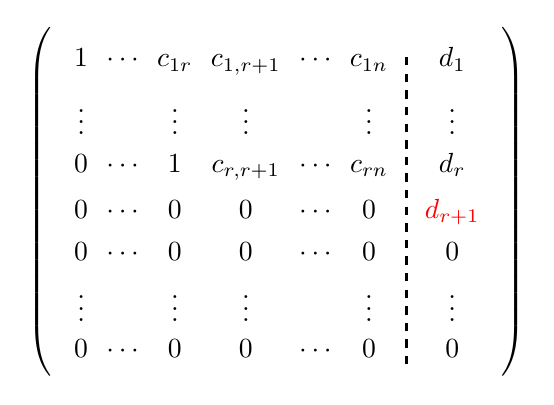
\begin{tikzpicture}
    \matrix(MM) [matrix of math nodes,nodes in empty cells,ampersand replacement=\&,left delimiter=(,right delimiter=)] {
      1\&\cd\&c_{1r}\&c_{1,r+1}\&\cd\&c_{1n}\&\&d_1\\        
      \vd\&\&\vd\&\vd\&\&\vd\&\&\vd\\
      0\&\cd\&1\&c_{r,r+1}\&\cd\&c_{rn}\&\&d_r\\
      0\&\cd\&0\&0\&\cd\&0\&\&\red{d_{r+1}}\\
      0\&\cd\&0\&0\&\cd\&0\&\&0\\        
      \vd\&\&\vd\&\vd\&\&\vd\&\&\vd\\
      0\&\cd\&0\&0\&\cd\&0\&\&0\\
    };  
    \draw[thick,dashed] (MM-1-7.north)--(MM-7-7.south);
  \end{tikzpicture}
\end{center}
其中$d_{r+1}\ne 0$(否则$\rank(\A,\bb)=r$)。这意味着出现了矛盾方程
$$
0 = \red{d_{r+1}}.
$$    
\end{frame}

\begin{frame}
\begin{tuilun}
  $$
  \A\xx=\bb\mbox{有唯一解} ~~\Longleftrightarrow~~
  \rank(\A,\bb)=\rank(\A)=\A\mbox{的列数}.
  $$
\end{tuilun}
\begin{center}
  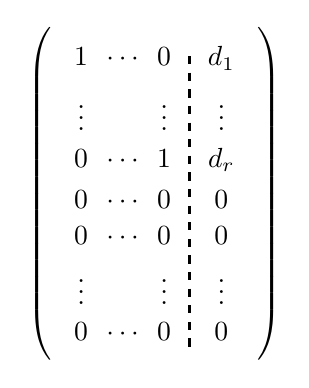
\begin{tikzpicture}
    \matrix(MM) [matrix of math nodes,nodes in empty cells,ampersand replacement=\&,left delimiter=(,right delimiter=)] {
      1\&\cd\&0\&\&d_1\\        
      \vd\&\&\vd\&\&\vd\\
      0\&\cd\&1\&\&d_r\\
      0\&\cd\&0\&\&0\\
      0\&\cd\&0\&\&0\\
      \vd\&\&\vd\&\&\vd\\
      0\&\cd\&0\&\&0\\
    };  
    \draw[thick,dashed] (MM-1-4.north)--(MM-7-4.south);
  \end{tikzpicture}
\end{center}
\end{frame}

\begin{frame}
\begin{dingli}
  若$\xx_1,~\xx_2$是$\A\xx=\bb$的解,则$\xx_1-\xx_2$是$\A\xx=\zero$的解。
\end{dingli}
\pause 
\begin{proof}
$$
\A(\xx_1-\xx_2)=\A\xx_1-\A\xx_2=\bb-\bb=\zero,
$$
故$\xx_1-\xx_2$是$\A\xx=\zero$的解。
\end{proof}
\end{frame}

\begin{frame}
\begin{dingli}
  若$\A\xx=\bb$有解,则其一般解(或称通解)为
  $$
  \xx=\xx_0+\bar\xx
  $$
  其中$\xx_0$是$\A\xx=\bb$的一个特解,而
  $$
  \bar\xx=k_1\xx_1+k_2\xx_2+\cd+k_p\xx_p
  $$
  为$\A\xx=\zero$的一般解。
\end{dingli}
\pause 
\begin{proof}
  $$
  \A(\xx_0+\bar\xx)=\A\xx_0+\A\bar\xx=\bb ~~\Rightarrow~~
  \xx_0+\bar\xx\mbox{是}\A\xx=\bb\mbox{的解}
  $$
  设$\xx^*$是$\A\xx=\bb$的任意一个解,则$\xx^*-\xx_0$是$\A\xx=\zero$的解,而
  $$
  \xx^*=\xx_0+(\xx^*-\xx_0).
  $$
  故$\xx^*$可表示为$\xx_0+\bar\xx$的形式。
\end{proof}
\end{frame}

\begin{frame}
非齐次线性方程组
$$\A\xx=\bb$$
的通解为
$$
k_1\xx_1+k_2\xx_2+\cd+k_p\xx_p + \red{\xx_0}
$$
其中$\xx_1,\xx_2,\cd,\xx_p$为$\A\xx=\zero$的基础解系,$\xx_0$为$\A\xx=\bb$的一个特解。
\end{frame}

\begin{frame}
\begin{zhu*}
  “$\A\xx=\bb$的通解” =  “$\A\xx=\zero$的通解” + “$\A\xx=\bb$的特解”
\end{zhu*}
\end{frame}

\begin{frame}
\begin{li}
  求非齐次线性方程组$\A\xx=\bb$的一般解,其中增广矩阵为
  $$
  (\A,\bb) = \left(
    \begin{array}{rrrrr}
      1&-1&-1& 1&\red{0}\\
      1&-1& 1&-3&\red{1}\\
      1&-1&-2& 3&\red{-\frac12}
    \end{array}
  \right)
  $$
\end{li}
\end{frame}

\begin{frame}[allowframebreaks]
\begin{jie}
  $$
  \begin{array}{rl}
    \left(
    \begin{array}{rrrrr}
      1&-1&-1& 1&\red{0}\\
      1&-1& 1&-3&\red{1}\\
      1&-1&-2& 3&\red{-\frac12}
    \end{array}
                  \right)  \xlongrightarrow[r_3-r_1]{r_2-r_1} &
                                                                \left(
                                                                \begin{array}{rrrrr}
                                                                  1&-1&-1& 1&\red{0}\\
                                                                  0& 0& 2&-4&\red{1}\\
                                                                  0& 0&-1& 2&\red{-\frac12}
                                                                \end{array}
                                                                              \right) \\[0.4in]
    \xlongrightarrow[r_2\div2]{r_1-r_3,r_3+\frac12r_2} &
                                                         \left(
                                                         \begin{array}{rrrrr}
                                                           1&-1&-1& 1&\red{0}\\
                                                           0& 0& 1&-2&\red{\frac12}\\
                                                           0& 0& 0& 0&\red{0}
                                                         \end{array}
                                                                       \right)
  \end{array}
  $$
  同解方程为
  $$
  \left\{
    \begin{array}{rcrcrcr}
      x_1&=&x_2&+&x_4&+&\frac12\\[0.1in]
      x_3&=&&&2x_4&+&\frac12
    \end{array}
  \right.
  $$
  亦即
  $$
  \left\{
    \begin{array}{rcrcrcr}
      x_1&=&x_2&+&x_4&+&\frac12\\[0.1in]
      x_2&=&x_2&&&&\\[0.1in]
      x_3&=&&&2x_4&+&\frac12\\[0.1in]
      x_4&=&&&x_4&&
    \end{array}
  \right.
  $$
  故通解为
  $$
  \left(
    \begin{array}{c}
      x_1\\x_2\\x_3\\x_4
    \end{array}
  \right) = c_1    \left(
    \begin{array}{c}
      1\\1\\0\\0
    \end{array}
  \right)+c_2    \left(
    \begin{array}{c}
      1\\0\\2\\1
    \end{array}
  \right)+    \left(
    \begin{array}{c}
      1/2\\0\\1/2\\0
    \end{array}
  \right) \quad c_1,c_2\in\mathbb R
  $$
\end{jie}
\end{frame}

\begin{frame}
\begin{li}[重要题型]
  设有线性方程组
  $$
  \left\{
    \begin{array}{rrrcr}
      (1+\lambda)x_1&+x_2&+x_3&=&0\\[0.05in]
      x_1&+(1+\lambda)x_2&+x_3&=&3\\[0.05in]
      x_1&+x_2&+(1+\lambda)x_3&=&\lambda
    \end{array}
  \right.
  $$
  问$\lambda$取何值时,此方程组
  \begin{itemize}
  \item[(1)]有唯一解?
  \item[(2)]无解? 
  \item[(3)]有无穷多解? 并在有无穷多解时求其通解。
  \end{itemize}
\end{li}
\end{frame}

\begin{frame}[allowframebreaks]
\begin{jie}
  $$
  |\A|=\left|
    \begin{array}{ccc}
      1+\lambda&1&1\\
      1&1+\lambda&1\\
      1&1&1+\lambda
    \end{array}
  \right| = (3+\lambda)\lambda^2.
  $$
  故当$\lambda\ne0$且$\lambda\ne-3$时,有唯一解。
  当$\lambda=0$时,原方程组为
  $$
  \left\{
    \begin{array}{l}
      x_1+x_2+x_3=0,\\
      x_1+x_2+x_3=3,\\
      x_1+x_2+x_3=0      
    \end{array}
  \right.
  $$
  它为矛盾方程组,故无解。 \vspace{0.1in}

  当$\lambda=-3$时,增广矩阵为
  $$
  \left(
    \begin{array}{rrrr}
      -2&1&1&\red{0}\\
      1&-2&1&\red{3}\\
      1&1&-2&\red{-3}
    \end{array}
  \right) \xlongrightarrow[]{\mbox{初等行变换}}
  \left(
    \begin{array}{rrrr}
      1&0&-1&\red{-1}\\
      0&1&-1&\red{-2}\\
      0&0&0&\red{0}
    \end{array}
  \right)
  $$
  得同解方程组为
  $$
  \left\{
    \begin{array}{l}
      x_1=x_3-1\\[0.05in]
      x_2=x_3-2\\[0.05in]
      x_3=x_3
    \end{array}
  \right.
  $$
  通解为
  $$
  \left(
    \begin{array}{c}
      x_1\\x_2\\x_3
    \end{array}
  \right) = c\left(
    \begin{array}{c}
      1\\1\\1
    \end{array}
  \right)+\left(
    \begin{array}{r}
      -1\\-2\\0
    \end{array}
  \right) \quad c\in\mathbb R
  $$
\end{jie}
\end{frame}

\begin{frame}
\begin{li}
  设$\etabd^*$为$\A\xx=\bb$的一个解,$\xibd_1,~\xibd_2,~\cd,~\xibd_{n-r}$为对应的齐次线性方程组的一个基础解系,证明:
  \begin{itemize}
  \item[(1)] $\etabd^*,~\xibd_1,~\xibd_2,~\cd,~\xibd_{n-r}$线性无关;
  \item[(2)] $\etabd^*,~\etabd^*+\xibd_1,~\etabd^*+\xibd_2,~\cd,~\etabd^*+\xibd_{n-r}$线性无关。
  \end{itemize}
\end{li}
\end{frame}

\begin{frame}
\begin{proof}
\begin{itemize}
\item[(1)] 假设$\etabd^*,~\xibd_1,~\xibd_2,~\cd,~\xibd_{n-r}$线性相关,而$\xibd_1,~\xibd_2,~\cd,~\xibd_{n-r}$线性无关,故$\etabd^*$可由$\xibd_1,~\xibd_2,~\cd,~\xibd_{n-r}$线性表示,从而$\etabd^*$为$\A\xx=\zero$的解,这与$\etabd^*$为$\A\xx=\bb$的解矛盾。故假设不成立,即$\etabd^*,~\xibd_1,~\xibd_2,~\cd,~\xibd_{n-r}$线性无关。 
\item[(2)] 显然,
  $$\etabd^*,~\xibd_1,~\xibd_2,~\cd,~\xibd_{n-r}
  \mbox{~~等价于~~} 
  \etabd^*,~\etabd^*+\xibd_1,~\etabd^*+\xibd_2,~\cd,~\etabd^*+\xibd_{n-r},$$  
  由题(1)结论可知
  $$
  \begin{aligned}
    &\rank(\etabd^*,~\etabd^*+\xibd_1,~\etabd^*+\xibd_2,~\cd,~\etabd^*+\xibd_{n-r})\\
    =& 
    \rank(\etabd^*,~\xibd_1,~\xibd_2,~\cd,~\xibd_{n-r}) = n-r+1
  \end{aligned}
  $$
  从而结论成立。
\end{itemize}
\end{proof}
\end{frame}

\begin{frame}
\begin{li}
  设$\etabd_1,~\etabd_2,~\cd,~\etabd_s$为$\A\xx=\bb$的$s$个解,$k_1,~k_2,~\cd,~k_{s}$为实数,满足$k_1+k_2+\cd+k_s=1$。证明:
  $$
  \xx=k_1\etabd_1+k_2\etabd_2+\cd+k_s\etabd_s
  $$
  也是它的解。
\end{li} \pause 
\begin{proof}
$$
\begin{array}{rcl}
  \A(k_1\etabd_1+k_2\etabd_2+\cd+k_{s}\etabd_{s})&=&
                                                     k_1\A\etabd_1+k_2\A\etabd_2+\cd+k_s\A\etabd_s\\[0.05in]
                                                 &=&k_1\bb+k_2\bb+\cd+k_s\bb\\[0.05in]
                                                 &=&\bb.
\end{array}
$$
\end{proof}
\end{frame}

\begin{frame}
\begin{li}
  对于$\A\xx=\bb$,$\rank(\A)=r$,$\etabd_1,~\etabd_2,~\cd,~\etabd_{n-r+1}$为它的$n-r+1$个线性无关的解。证明它的任一解可表示为
  $$
  \xx=k_1\etabd_1+k_2\etabd_2+\cd+k_{n-r+1}\etabd_{n-r+1},
  $$
  其中$k_1+k_2+\cd+k_{n-r+1}=1$
\end{li}
\end{frame}

\begin{frame}[allowframebreaks]
\begin{proof}
取向量组
$
\blue{\etabd_2-\etabd_1,~~\etabd_2-\etabd_1,~~\cd,~\etabd_{n-r+1}-\etabd_1.}
$
下证该向量组为$\A\xx=\zero$的一个基础解系。 
$$
(\etabd_1,~\etabd_2,~\cd,~\etabd_{n-r+1}) \xlongrightarrow[j=2,\cd,n-r+1]{c_j-c_1}
(\etabd_1,~\etabd_2-\etabd_1,~\cd,~\etabd_{n-r+1}-\etabd_1)
$$ 
$$
\begin{array}{rl}
  &\etabd_1,~\etabd_2,~\cd,~\etabd_{n-r+1}\mbox{线性无关}\\[0.1in]  
  \Rightarrow&\etabd_1,~\etabd_2-\etabd_1,~\cd,~\etabd_{n-r+1}-\etabd_1\mbox{线性无关}\\[0.1in]  
  \Rightarrow&\etabd_2-\etabd_1,~\cd,~\etabd_{n-r+1}-\etabd_1\mbox{线性无关}\\[0.1in]  
  \Rightarrow& \etabd_2-\etabd_1,~\cd,~\etabd_{n-r+1}-\etabd_1\mbox{为}\A\xx=\zero
               \mbox{的基础解系}.      
\end{array}
$$
于是$\A\xx=\bb$的任意一个解$\xx$可表示为
$$
\begin{array}{rl}
  & \xx = k_2(\etabd_2-\etabd_1)+\cd+k_{n-r+1}(\etabd_{n-r+1}-\etabd_1)+\red{\etabd_1}\\[0.1in] 
  \Rightarrow & 
                \xx = (1-k_2-\cd-k_{n+r-1})\etabd_1+k_2\etabd_2+\cd+k_{n-r+1}\etabd_{n-r+1}\\[0.1in]
  \Rightarrow & 
                \xx =k_1\etabd_1+k_2\etabd_2+\cd+k_{n-r+1}\etabd_{n-r+1}
\end{array}
$$
\end{proof}
\end{frame}


\begin{frame}
\begin{li}
  设四元齐次线性方程组
  $$
  (I):\left\{
    \begin{array}{l}
      x_1+x_2=0,\\
      x_2-x_4=0;
    \end{array}
  \right. \quad
  (II):\left\{
    \begin{array}{l}
      x_1-x_2+x_3=0,\\
      x_2-x_3+x_4=0.
    \end{array}
  \right.
  $$
  求
  \begin{itemize}
  \item[(1)] 方程组$(I)$与$(II)$的基础解系
  \item[(2)] 方程组$(I)$与$(II)$的公共解        
  \end{itemize}
\end{li}
\end{frame}

\begin{frame}
\begin{jie}
  (1)、因为
    $$
    (I) \Longleftrightarrow
    \left\{
      \begin{array}{rcr}
        x_1&=&-x_2\\[0.05in]
        x_4&=&x_2
      \end{array}
    \right. \Longleftrightarrow
    \left\{
      \begin{array}{rcrr}
        x_1&=&-x_2&\\[0.05in]
        x_2&=&x_2&\\[0.05in]
        x_3&=&&x_3\\[0.05in]
        x_4&=&x_2&
      \end{array}
    \right. 
    $$   
    故$(I)$的基础解系为
    $$
    \xibd_1=\left(
      \begin{array}{r}
        -1\\1\\0\\1
      \end{array}
    \right), \quad
    \xibd_2=\left(
      \begin{array}{r}
        0\\0\\1\\0
      \end{array}
    \right)
    $$
  \end{jie}
  \end{frame}

\begin{frame}
\begin{jie}[续]
  因为
  $$
  (II) \Longleftrightarrow
  \left\{
    \begin{array}{rcrr}
      x_1&=&x_2&-x_3\\[0.05in]
      x_4&=&-x_2&+x_3
    \end{array}
  \right. \Longleftrightarrow
  \left\{
    \begin{array}{rcrr}
      x_1&=&x_2&-x_3\\[0.05in]
      x_2&=&x_2&\\[0.05in]
      x_3&=&&x_3\\[0.05in]
      x_4&=&-x_2&+x_3
    \end{array}
  \right. 
  $$
  故$(II)$的基础解系为
  $$
  \xibd_1=\left(
    \begin{array}{r}
      1\\1\\0\\-1
    \end{array}
  \right), \quad
  \xibd_2=\left(
    \begin{array}{r}
      -1\\0\\1\\1
    \end{array}
  \right)
  $$
\end{jie}
\end{frame}

\begin{frame}
\begin{jie}[续]
  (2)、 方程$(I)$与$(II)$的公共解即为联立$(I)$与$(II)$所得新方程组的解:
    $$
    \left\{
      \begin{array}{l}
        x_1+x_2=0\\
        x_2-x_4=0\\
        x_1-x_2+x_3=0\\
        x_2-x_3+x_4=0
      \end{array}
    \right.
    $$
\end{jie}
\end{frame}

\begin{frame}
\begin{jie}[续]

    $$
    \begin{array}{rl}
      \left(
      \begin{array}{rrrr}
        1&1&0&0\\
        0&1&0&-1\\
        1&-1&1&0\\
        0&1&-1&1
      \end{array}
                \right) \xlongrightarrow[r_3-r_1]{r_4+r_2} & 
                                                             \left(
                                                             \begin{array}{rrrr}
                                                               1&1&0&0\\
                                                               0&1&0&-1\\
                                                               0&-2&1&0\\
                                                               0&2&-1&0
                                                             \end{array}
                                                                       \right) \\[0.3in]
      \xlongrightarrow[r_3\times(-1)]{r_3+r_4}&
                                                \left(
                                                \begin{array}{rrrr}
                                                  1&1&0&0\\
                                                  0&1&0&-1\\
                                                  0&2&-1&0\\
                                                  0&0&0&0
                                                \end{array}
                                                         \right)         
    \end{array}
    $$  
    即
    $$
    \left\{
      \begin{array}{rcr}
        x_1&=&-x_2\\
        x_2&=&x_2\\
        x_3&=&2x_2\\
        x_4&=&x_2
      \end{array}
    \right.  ~~ \Rightarrow ~~
    \xx = c\left(
      \begin{array}{r}
        -1\\1\\2\\1
      \end{array}
    \right) \quad c\in \mathbb R.
    $$
\end{jie}
\end{frame}








\end{CJK}
\end{document}

